\documentclass[11pt,a4paper]{article}

\usepackage[utf8]{inputenc}
\usepackage[T1]{fontenc}
\usepackage[brazilian]{babel}
\usepackage{geometry}
\geometry{margin=2.5cm}

\usepackage{graphicx}
\usepackage{float}
\usepackage{booktabs}
\usepackage{pgfplots}
\pgfplotsset{compat=1.18}
\usepackage{xcolor}
\usepackage{hyperref}
\usepackage{cleveref}

\title{Análise da Atividade de Code Review no GitHub}
\author{Érica Alves dos Santos \and Gustavo Pimentel Carvalho Costa}
\date{\today}

\usepackage{xspace}
\newcommand{\spearman}{Spearman\xspace}


\begin{document}
\maketitle

\begin{abstract}
Este trabalho analisa 9.075 Pull Requests de 197 repositórios populares do GitHub,
investigando relações entre tamanho, tempo de análise, descrição e interações
com o status de merge e número de revisões. Utilizamos correlação de \spearman
e testes de significância para responder a sete questões de pesquisa.
Os resultados indicam que o tempo de análise é o fator mais fortemente associado
ao status de merge, enquanto o tamanho do PR apresenta correlação moderada
com o número de revisões.
\end{abstract}

\section{Introdução}
A prática de code review tornou-se uma constante nos processos de desenvolvimento
ágeis. No contexto de sistemas open source, as atividades de code review
acontecem a partir da avaliação de contribuições submetidas por meio de
Pull Requests (PR). Este trabalho tem como objetivo analisar a atividade de
code review desenvolvida em repositórios populares do GitHub, identificando
variáveis que influenciam no merge de um PR.

Investigamos sete questões de pesquisa organizadas em duas dimensões:
\begin{itemize}
    \item \textbf{Dimensão A:} relação entre características do PR e seu status final (merged ou closed);
    \item \textbf{Dimensão B:} relação entre características do PR e o número de revisões realizadas.
\end{itemize}

As características analisadas são: tamanho (arquivos e linhas alteradas),
tempo de análise, descrição (número de caracteres) e interações
(número de participantes).


\section{Metodologia}
\subsection{Seleção de Repositórios}

Foram selecionados 197 repositórios populares do GitHub, extraídos da busca
pública ordenada por estrelas. Critérios de inclusão: pelo menos 100 PRs fechados.

\subsection{Seleção de Pull Requests}

Foram analisados 9.075 PRs que atendem aos seguintes critérios:
\begin{itemize}
    \item Status MERGED ou CLOSED;
    \item Pelo menos uma revisão oficial (campo \texttt{review\_count} $\geq$ 1);
    \item Tempo de análise maior que 1 hora.
\end{itemize}

\subsection{Métricas}

As métricas extraídas para cada PR são:
\begin{itemize}
    \item \textbf{Tamanho:} número de arquivos modificados e total de linhas alteradas;
    \item \textbf{Tempo de Análise:} intervalo entre criação e fechamento/merge (horas);
    \item \textbf{Descrição:} número de caracteres do corpo do PR;
    \item \textbf{Interações:} número de participantes distintos;
    \item \textbf{Revisões:} número de submissões de revisão oficiais.
\end{itemize}

\textbf{Nota:} os campos \texttt{comments\_count} e \texttt{review\_comments\_count}
apresentaram valores zerados na coleta. Como proxy para interações,
utilizamos o número de participantes, que foi corretamente coletado.

\subsection{Testes Estatísticos}

Utilizamos o coeficiente de correlação de \spearman ($\rho$), um método
não-paramétrico robusto a outliers e distribuições não-normais.
Aplicamos winsorização no percentil 99 para mitigar o impacto de outliers extremos.

O nível de significância adotado foi $\alpha = 0.05$. A magnitude do efeito
foi classificada conforme o valor de $|\rho|$:
desprezível ($<$0,1), fraca (0,1--0,3), moderada (0,3--0,5), forte (0,5--0,7),
muito forte ($>$0,7).

\subsection{Visualizações}

Para a representação gráfica, seguimos as recomendações de Claus O. Wilke
(\textit{Fundamentals of Data Visualization}, O'Reilly, 2019):
\begin{itemize}
    \item \textbf{ECDF} (Função de Distribuição Cumulativa Empírica) para comparações
    de distribuição entre grupos (Dimensão A), por ser livre de parâmetros arbitrários
    (como largura de bins em histogramas) e robusta a outliers.
    \item \textbf{Violin plots com boxplot interno} para relações entre variável contínua
    e discreta (Dimensão B), revelando a distribuição completa sem adicionar ruído artificial.
    \item \textbf{Matriz de correlação triangular} para visão geral das relações
    entre todas as métricas.
\end{itemize}


\section{Resultados}
\subsection{Estatísticas Descritivas}

A \cref{tab:desc} apresenta as estatísticas descritivas das métricas analisadas.

\begin{table}[h]
\centering
\caption{Estatísticas Descritivas}
\label{tab:desc}
\begin{tabular}{lrrrrrrrr}
\toprule
Metrica & Count & Mean & Std & Min & 25\% & Median & 75\% & Max \\
\midrule
files\_changed & 9075.0 & 6.9 & 18.2 & 1.0 & 1.0 & 2.0 & 5.0 & 143.3 \\
lines\_added & 9075.0 & 385.2 & 1512.5 & 0.0 & 2.0 & 20.0 & 124.0 & 12194.7 \\
lines\_deleted & 9075.0 & 94.1 & 414.4 & 0.0 & 1.0 & 3.0 & 19.0 & 3403.7 \\
total\_changes & 9075.0 & 576.2 & 2437.6 & 1.0 & 4.0 & 30.0 & 168.0 & 20171.9 \\
analysis\_time\_hours & 9075.0 & 2105.0 & 6020.9 & 1.2 & 16.6 & 101.6 & 887.8 & 37134.4 \\
description\_chars & 9075.0 & 1320.1 & 1998.3 & 0.0 & 130.0 & 670.0 & 1643.0 & 12038.9 \\
participants & 9075.0 & 3.5 & 1.7 & 2.0 & 2.0 & 3.0 & 4.0 & 11.0 \\
comments\_count & 9075.0 & 0.0 & 0.0 & 0.0 & 0.0 & 0.0 & 0.0 & 0.0 \\
review\_comments\_count & 9075.0 & 0.0 & 0.0 & 0.0 & 0.0 & 0.0 & 0.0 & 0.0 \\
total\_interactions & 9075.0 & 0.0 & 0.0 & 0.0 & 0.0 & 0.0 & 0.0 & 0.0 \\
review\_count & 9075.0 & 2.8 & 3.9 & 1.0 & 1.0 & 1.0 & 3.0 & 26.0 \\
\bottomrule
\end{tabular}

\end{table}

\subsection{Correlações por Questão de Pesquisa}

A \cref{tab:corr} resume os resultados das correlações de \spearman.

\begin{table}[h]
\centering
\caption{Resultados de Correlação}
\label{tab:corr}
\begin{tabular}{lccrrl}
\toprule
RQ & Variavel X & Variavel Y & $\rho$ & p-valor & Efeito \\
\midrule
RQ01 & total\_changes & merged & 0.0034 & 0.7475 & desprezivel \\
RQ02 & analysis\_time\_hours & merged & -0.3910 & 0.0000 & moderada \\
RQ03 & description\_chars & merged & -0.0288 & 0.0061 & desprezivel \\
RQ04 & participants & merged & -0.0756 & 0.0000 & desprezivel \\
RQ05 & total\_changes & review\_count & 0.3114 & 0.0000 & moderada \\
RQ06 & analysis\_time\_hours & review\_count & 0.0917 & 0.0000 & desprezivel \\
RQ07 & description\_chars & review\_count & 0.1861 & 0.0000 & fraca \\
\bottomrule
\end{tabular}

\end{table}

\subsection{Dimensão A: Status do PR}

\subsubsection{RQ01 -- Tamanho vs. Status}
A correlação entre tamanho do PR e status de merge é desprezível
($\rho = 0,0034$, $p = 0,7475$), não significativa.
Medianas idênticas (30 linhas alteradas) para merged e closed.

\begin{figure}[H]
    \centering
    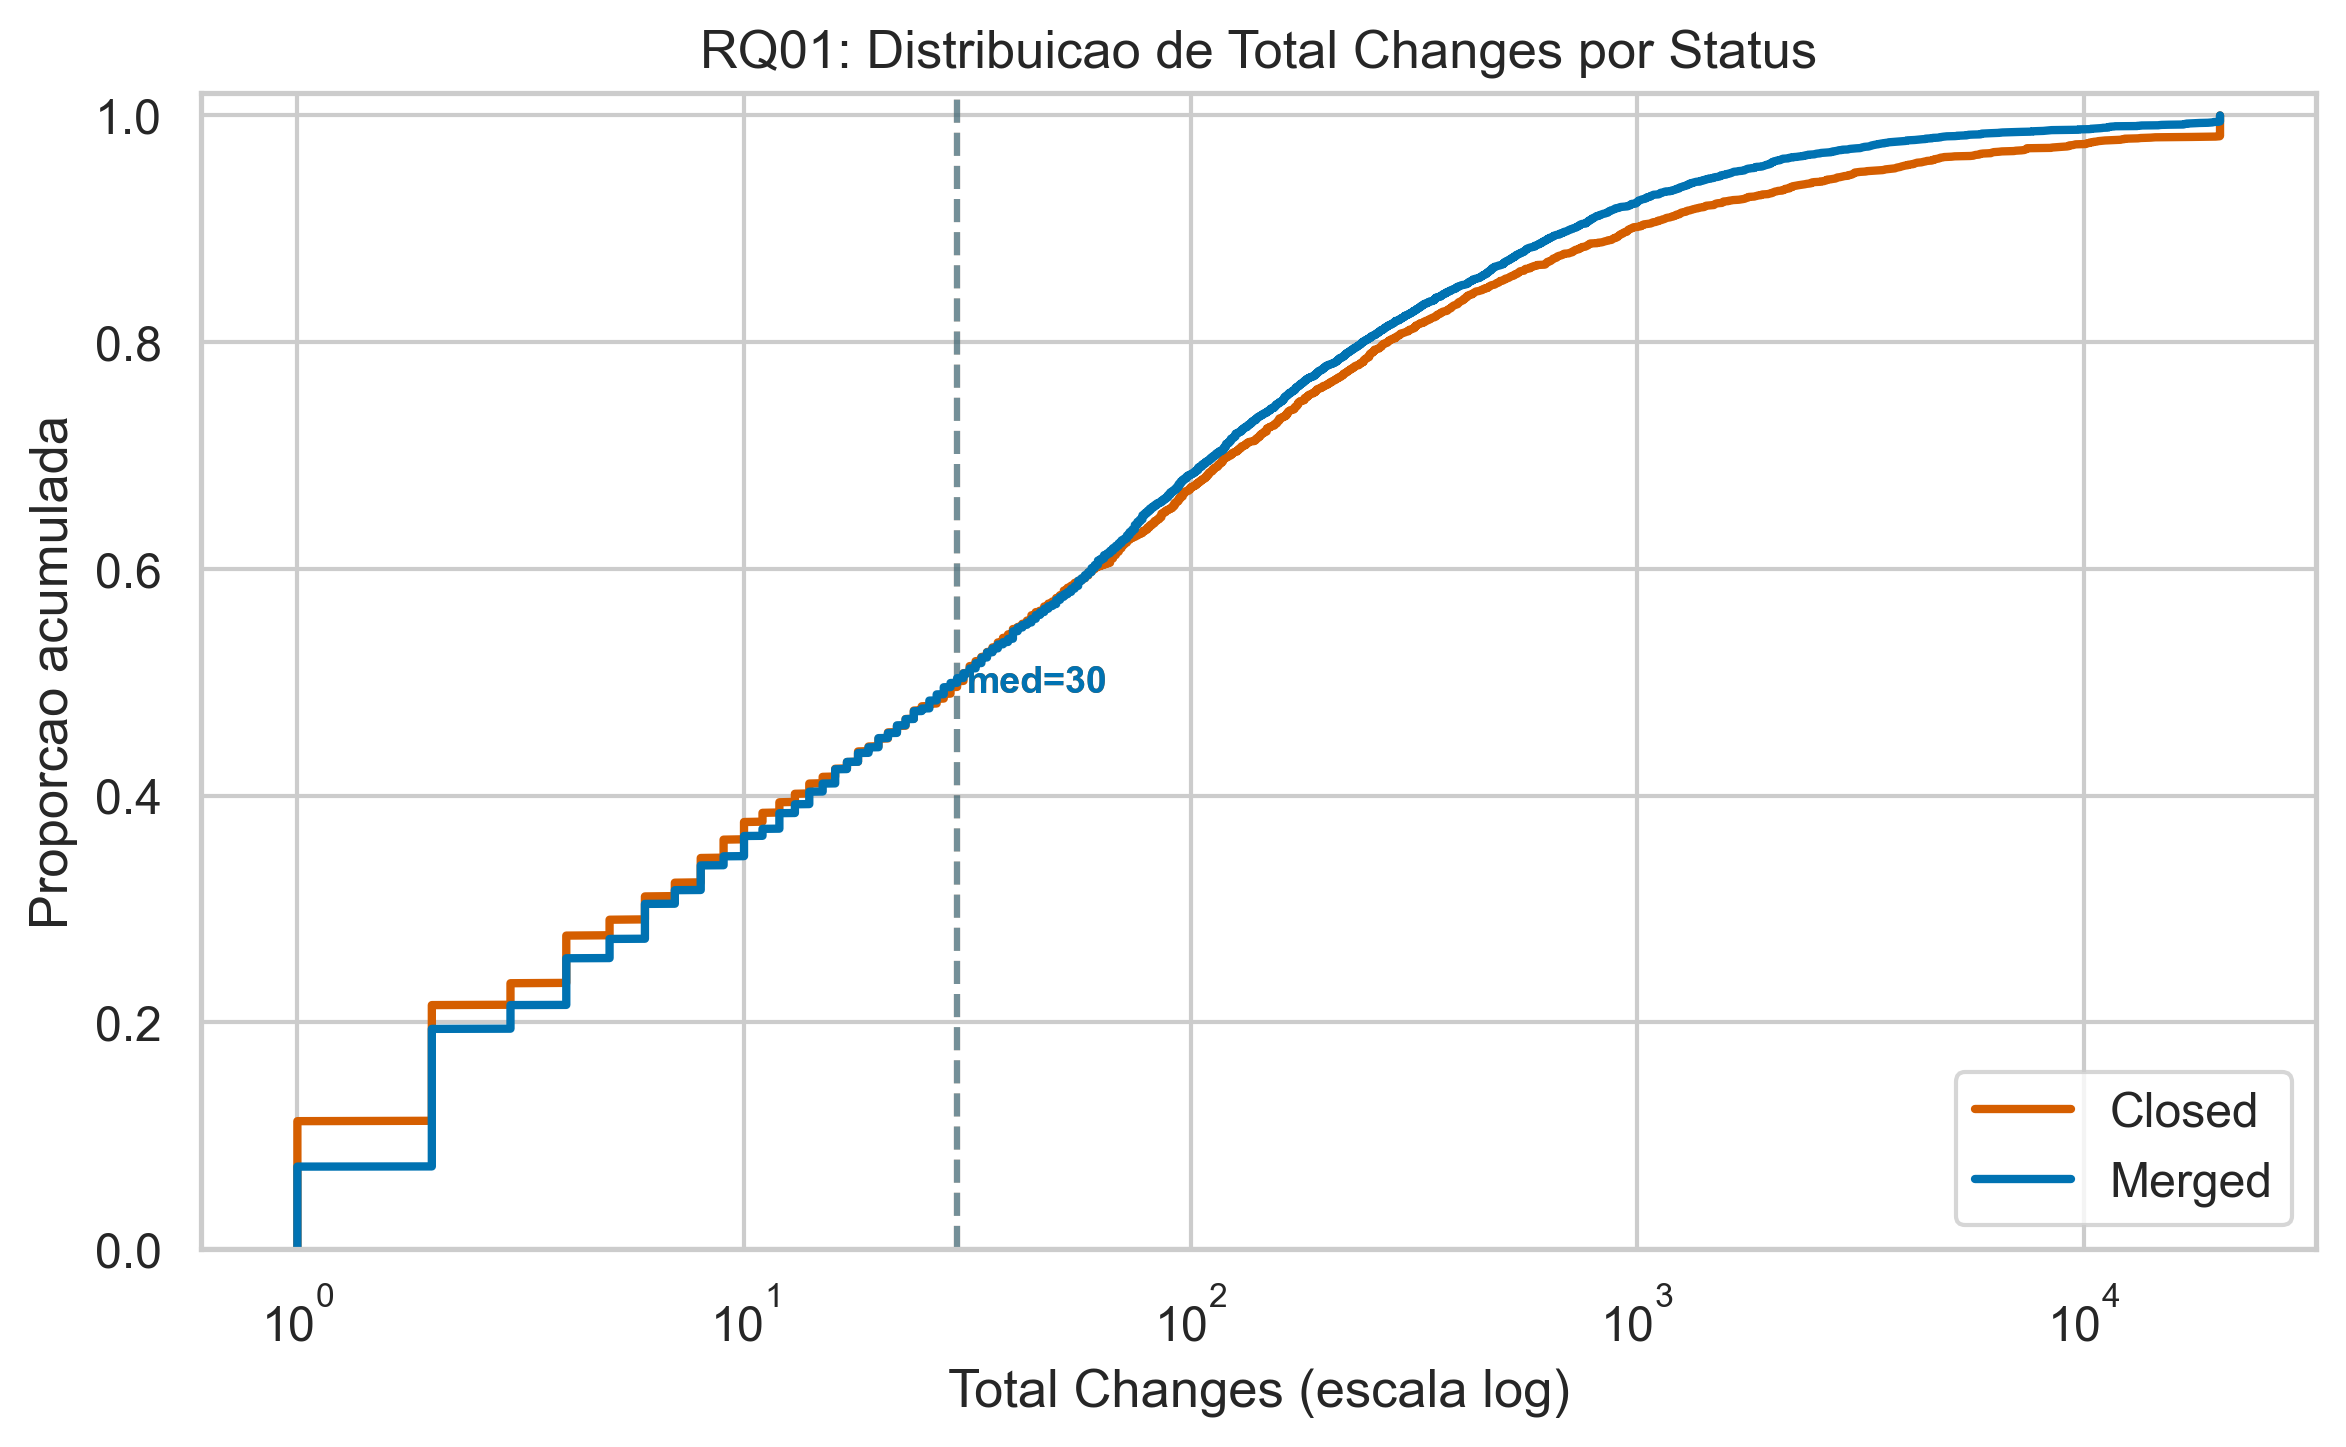
\includegraphics[width=0.85\textwidth]{figures/rq01.png}
    \caption{RQ01: ECDF do tamanho do PR por status de merge.}
    \label{fig:rq01}
\end{figure}

\subsubsection{RQ02 -- Tempo de Análise vs. Status}
Correlação moderada e negativa ($\rho = -0,3910$, $p < 0,0001$).
PRs merged tendem a ter menor tempo de análise: mediana de 47h para merged
vs 748h para closed.

\begin{figure}[H]
    \centering
    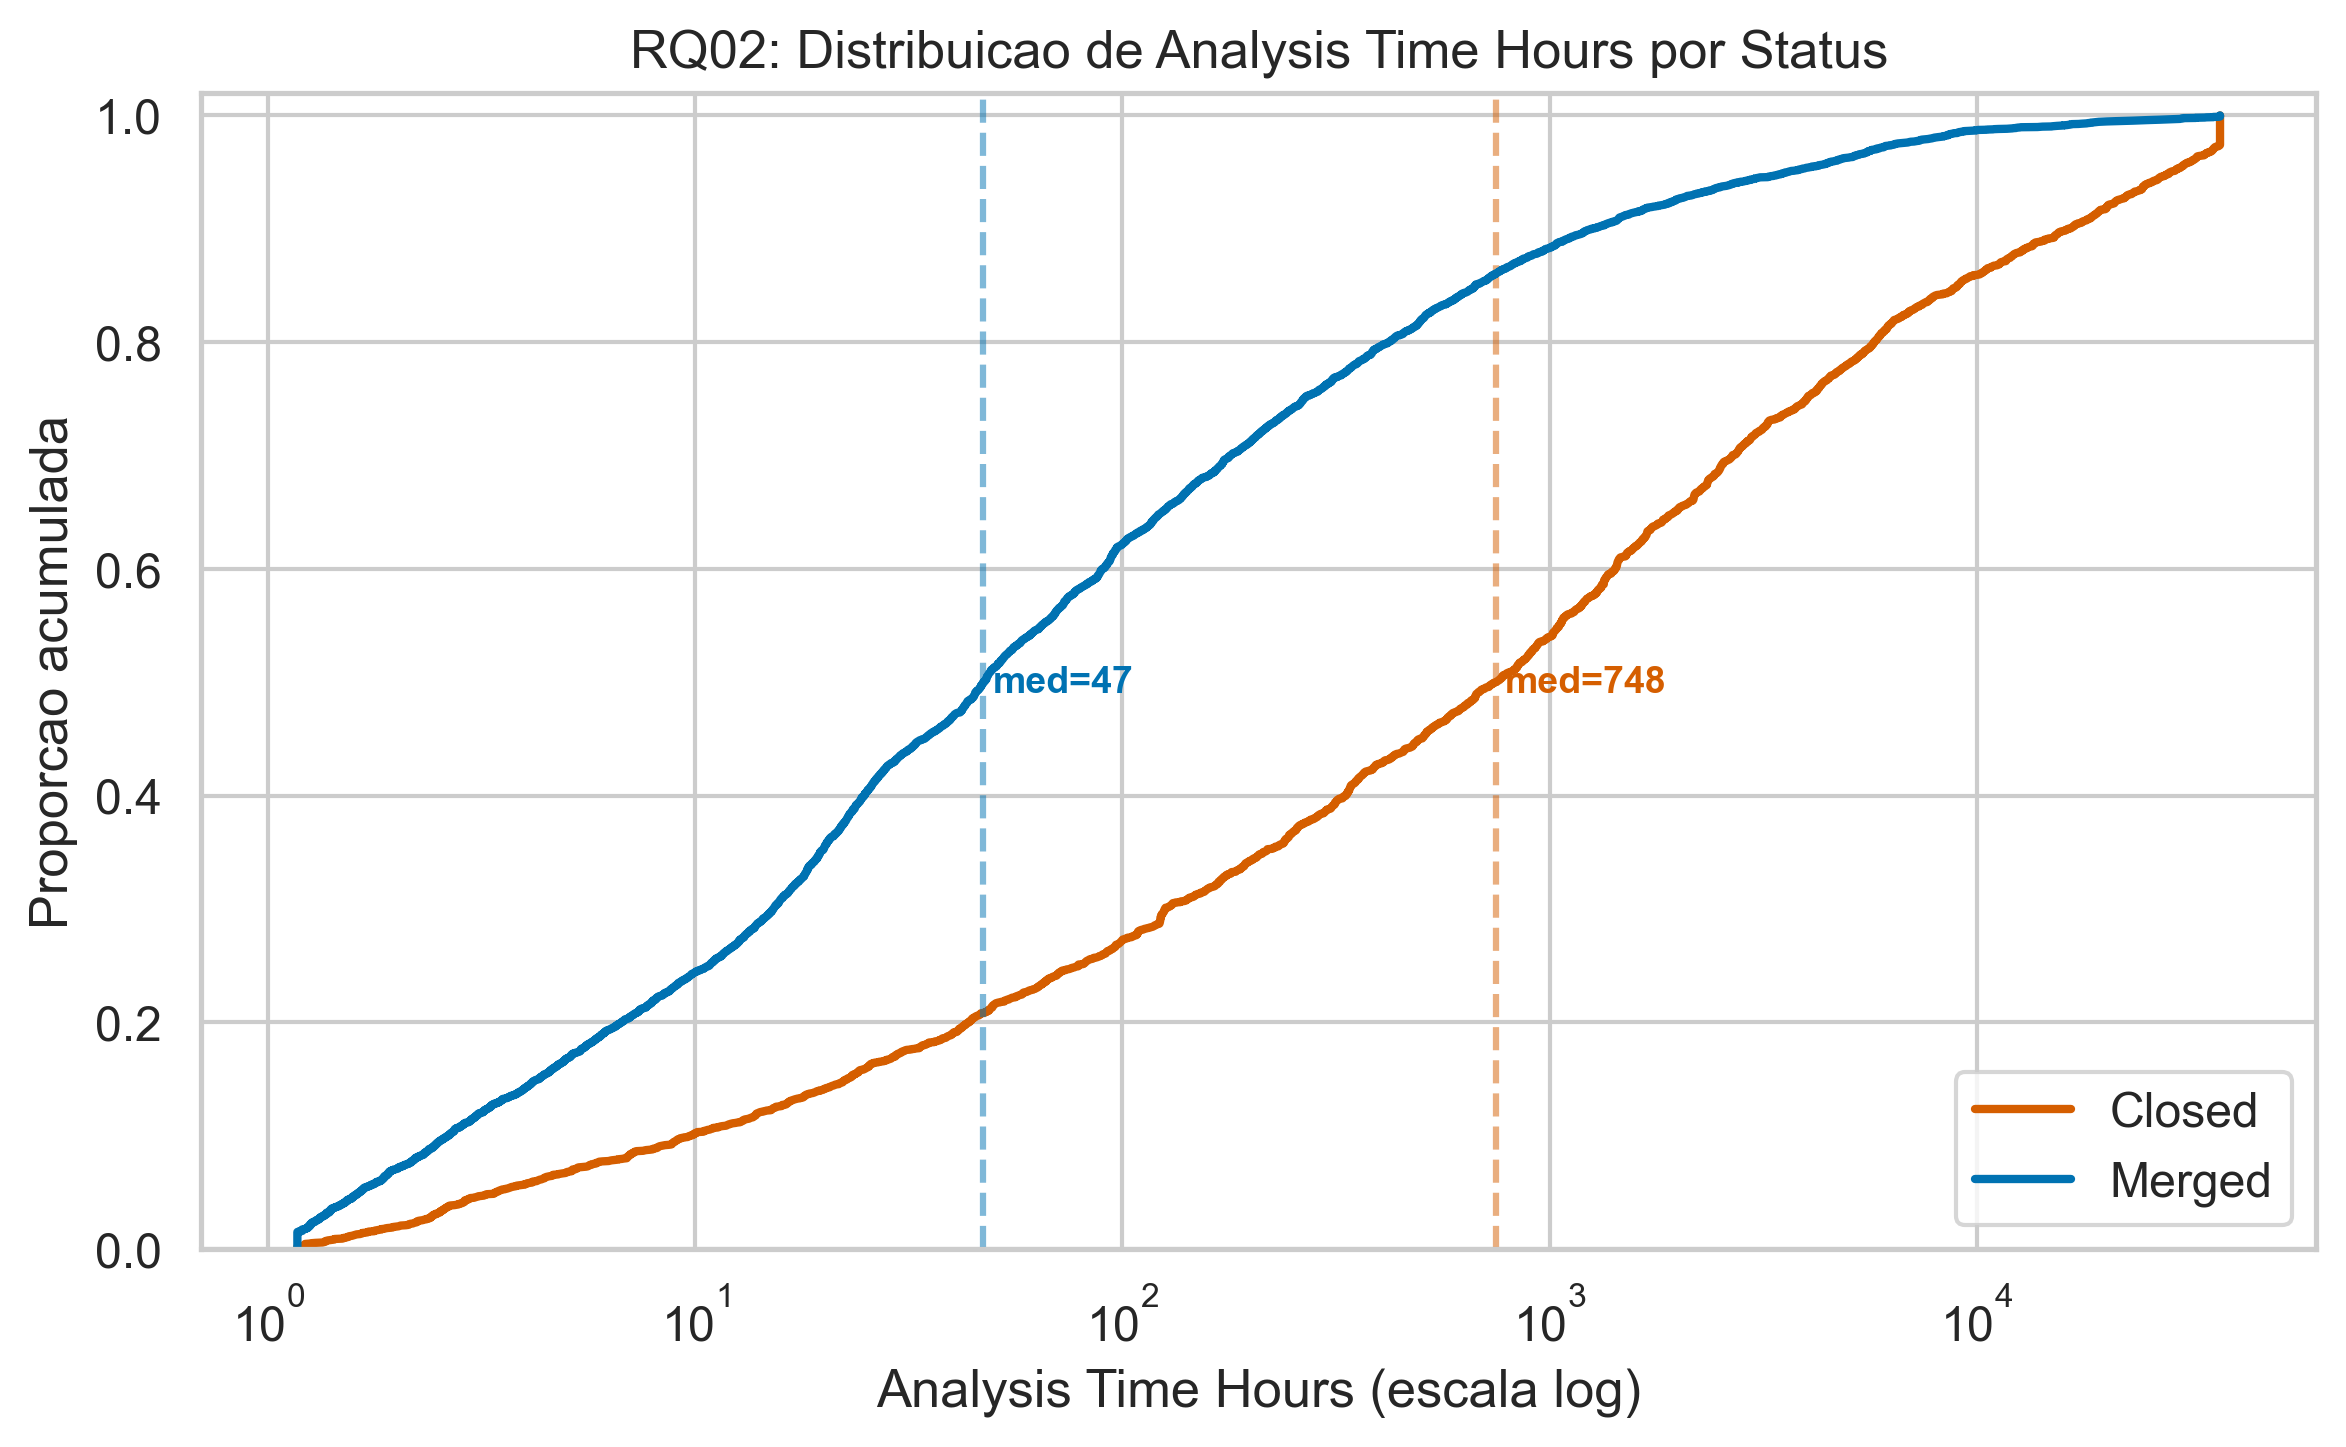
\includegraphics[width=0.85\textwidth]{figures/rq02.png}
    \caption{RQ02: ECDF do tempo de análise por status de merge.}
    \label{fig:rq02}
\end{figure}

\subsubsection{RQ03 -- Descrição vs. Status}
Correlação desprezível ($\rho = -0,0288$, $p = 0,0061$).
Apesar de significativa pelo tamanho da amostra, o efeito é praticamente nulo.

\begin{figure}[H]
    \centering
    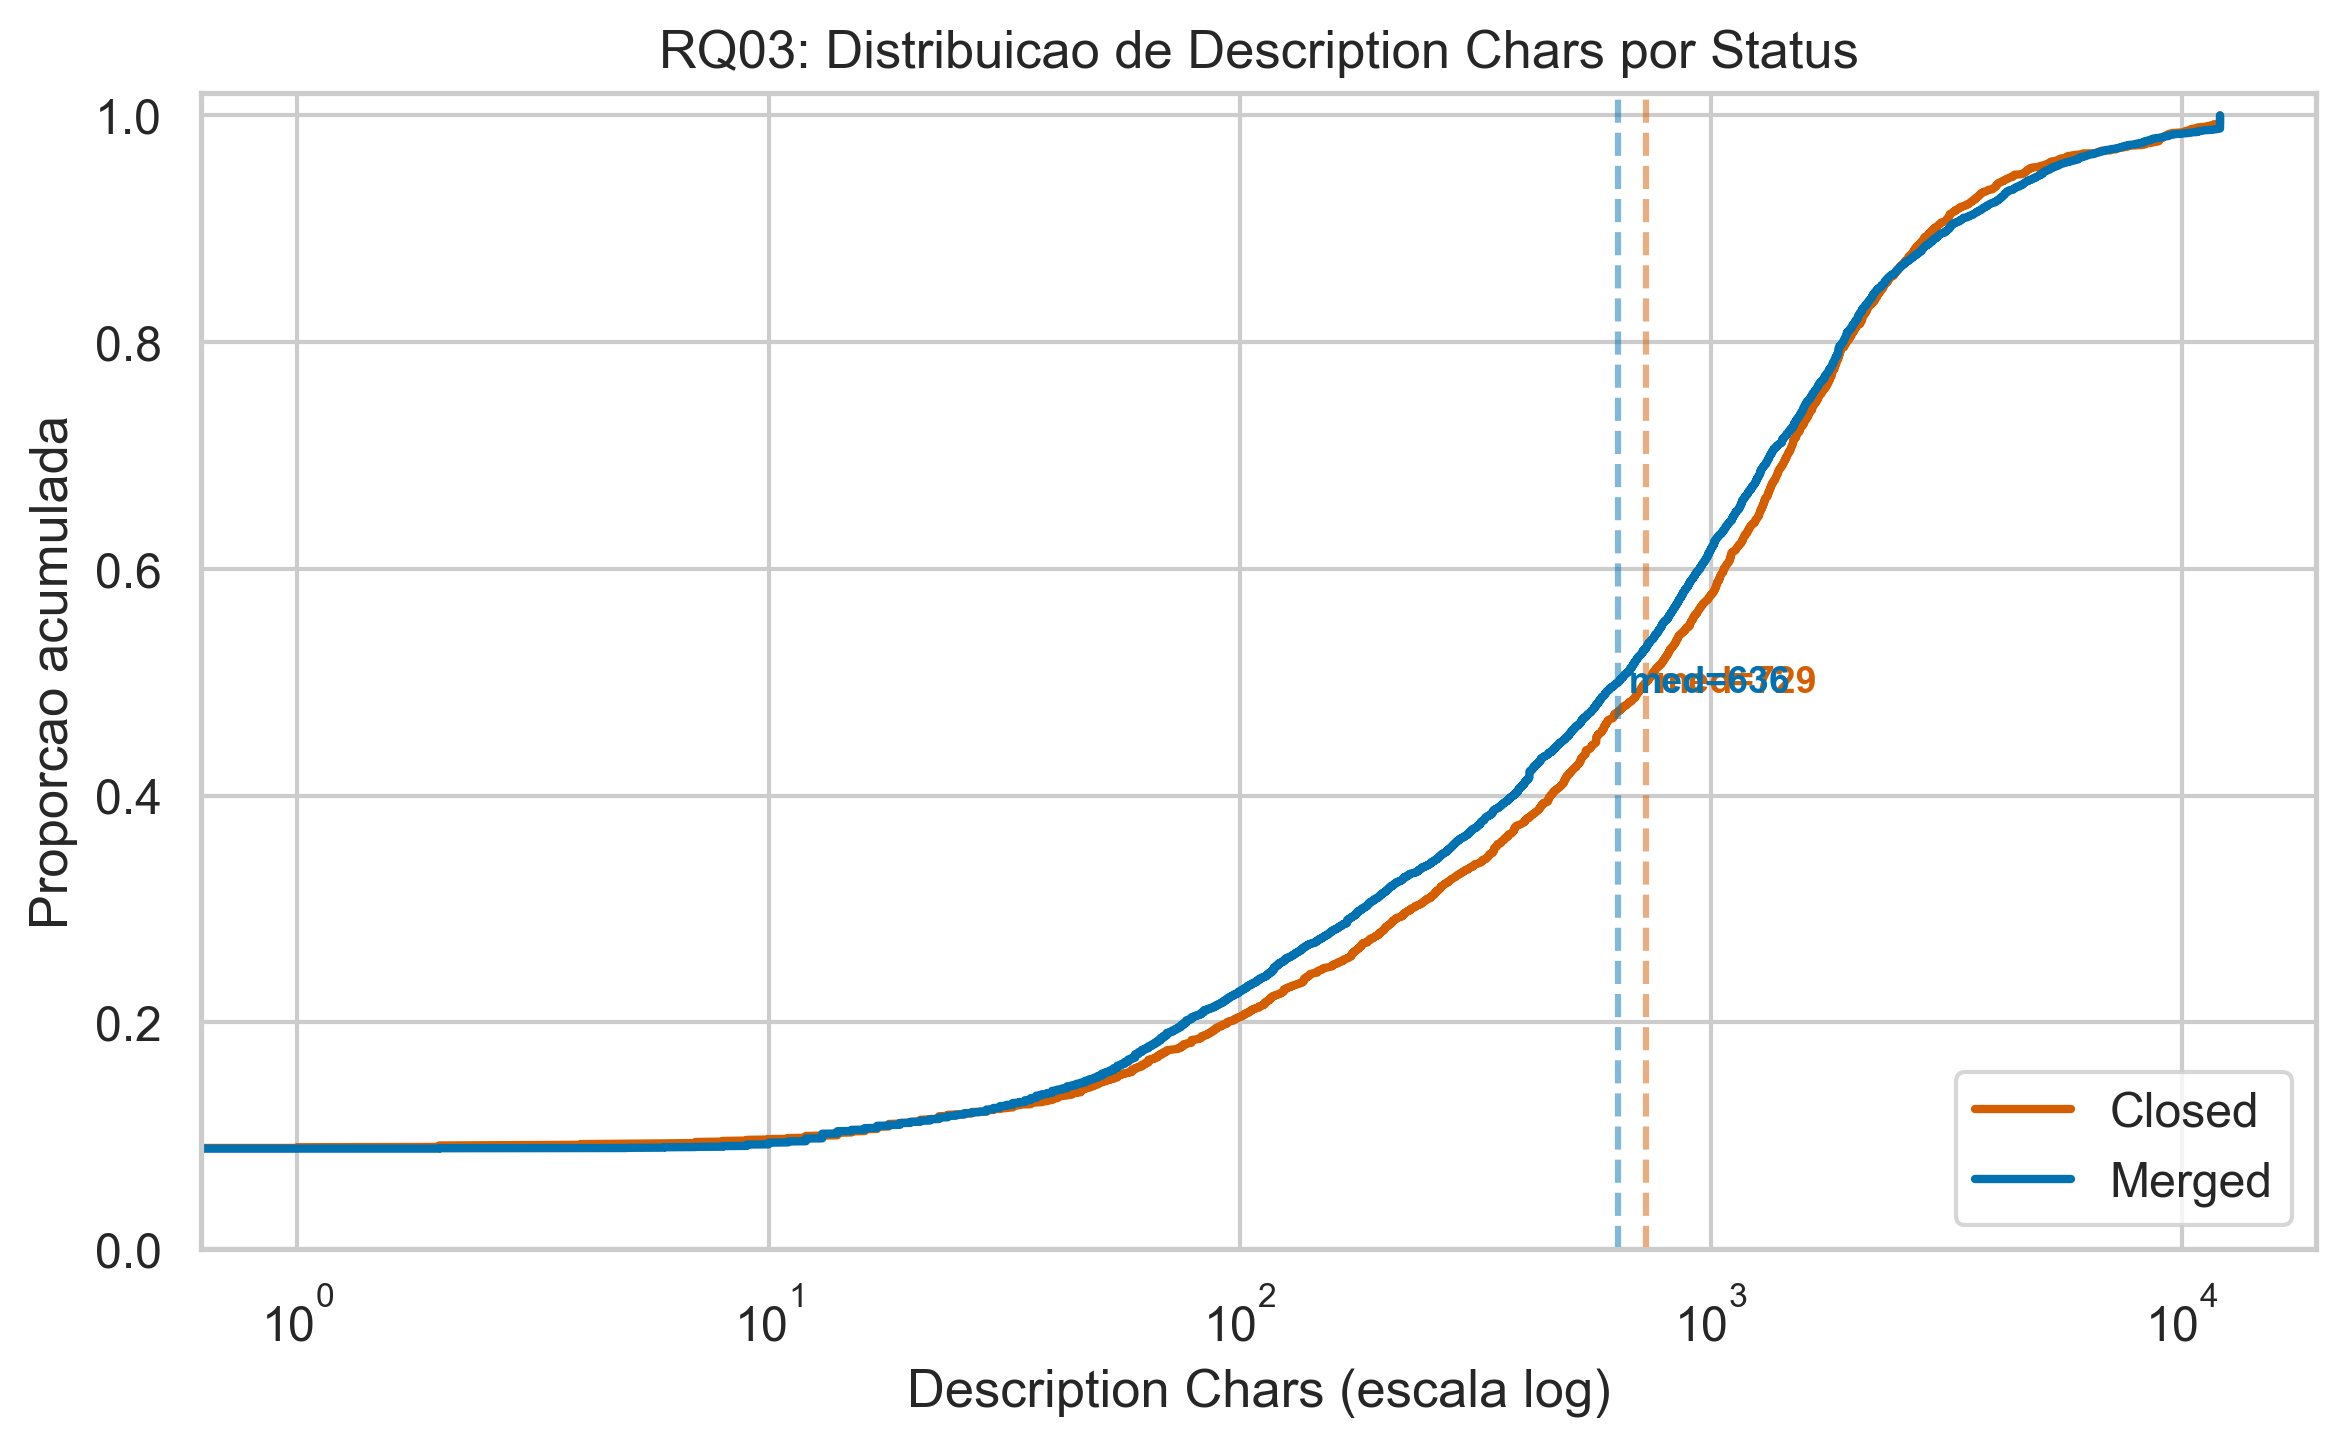
\includegraphics[width=0.85\textwidth]{figures/rq03.png}
    \caption{RQ03: ECDF do tamanho da descrição por status de merge.}
    \label{fig:rq03}
\end{figure}

\subsubsection{RQ04 -- Participantes vs. Status}
Correlação desprezível ($\rho = -0,0756$, $p < 0,0001$).
Mais participantes levemente associados a PRs closed.

\begin{figure}[H]
    \centering
    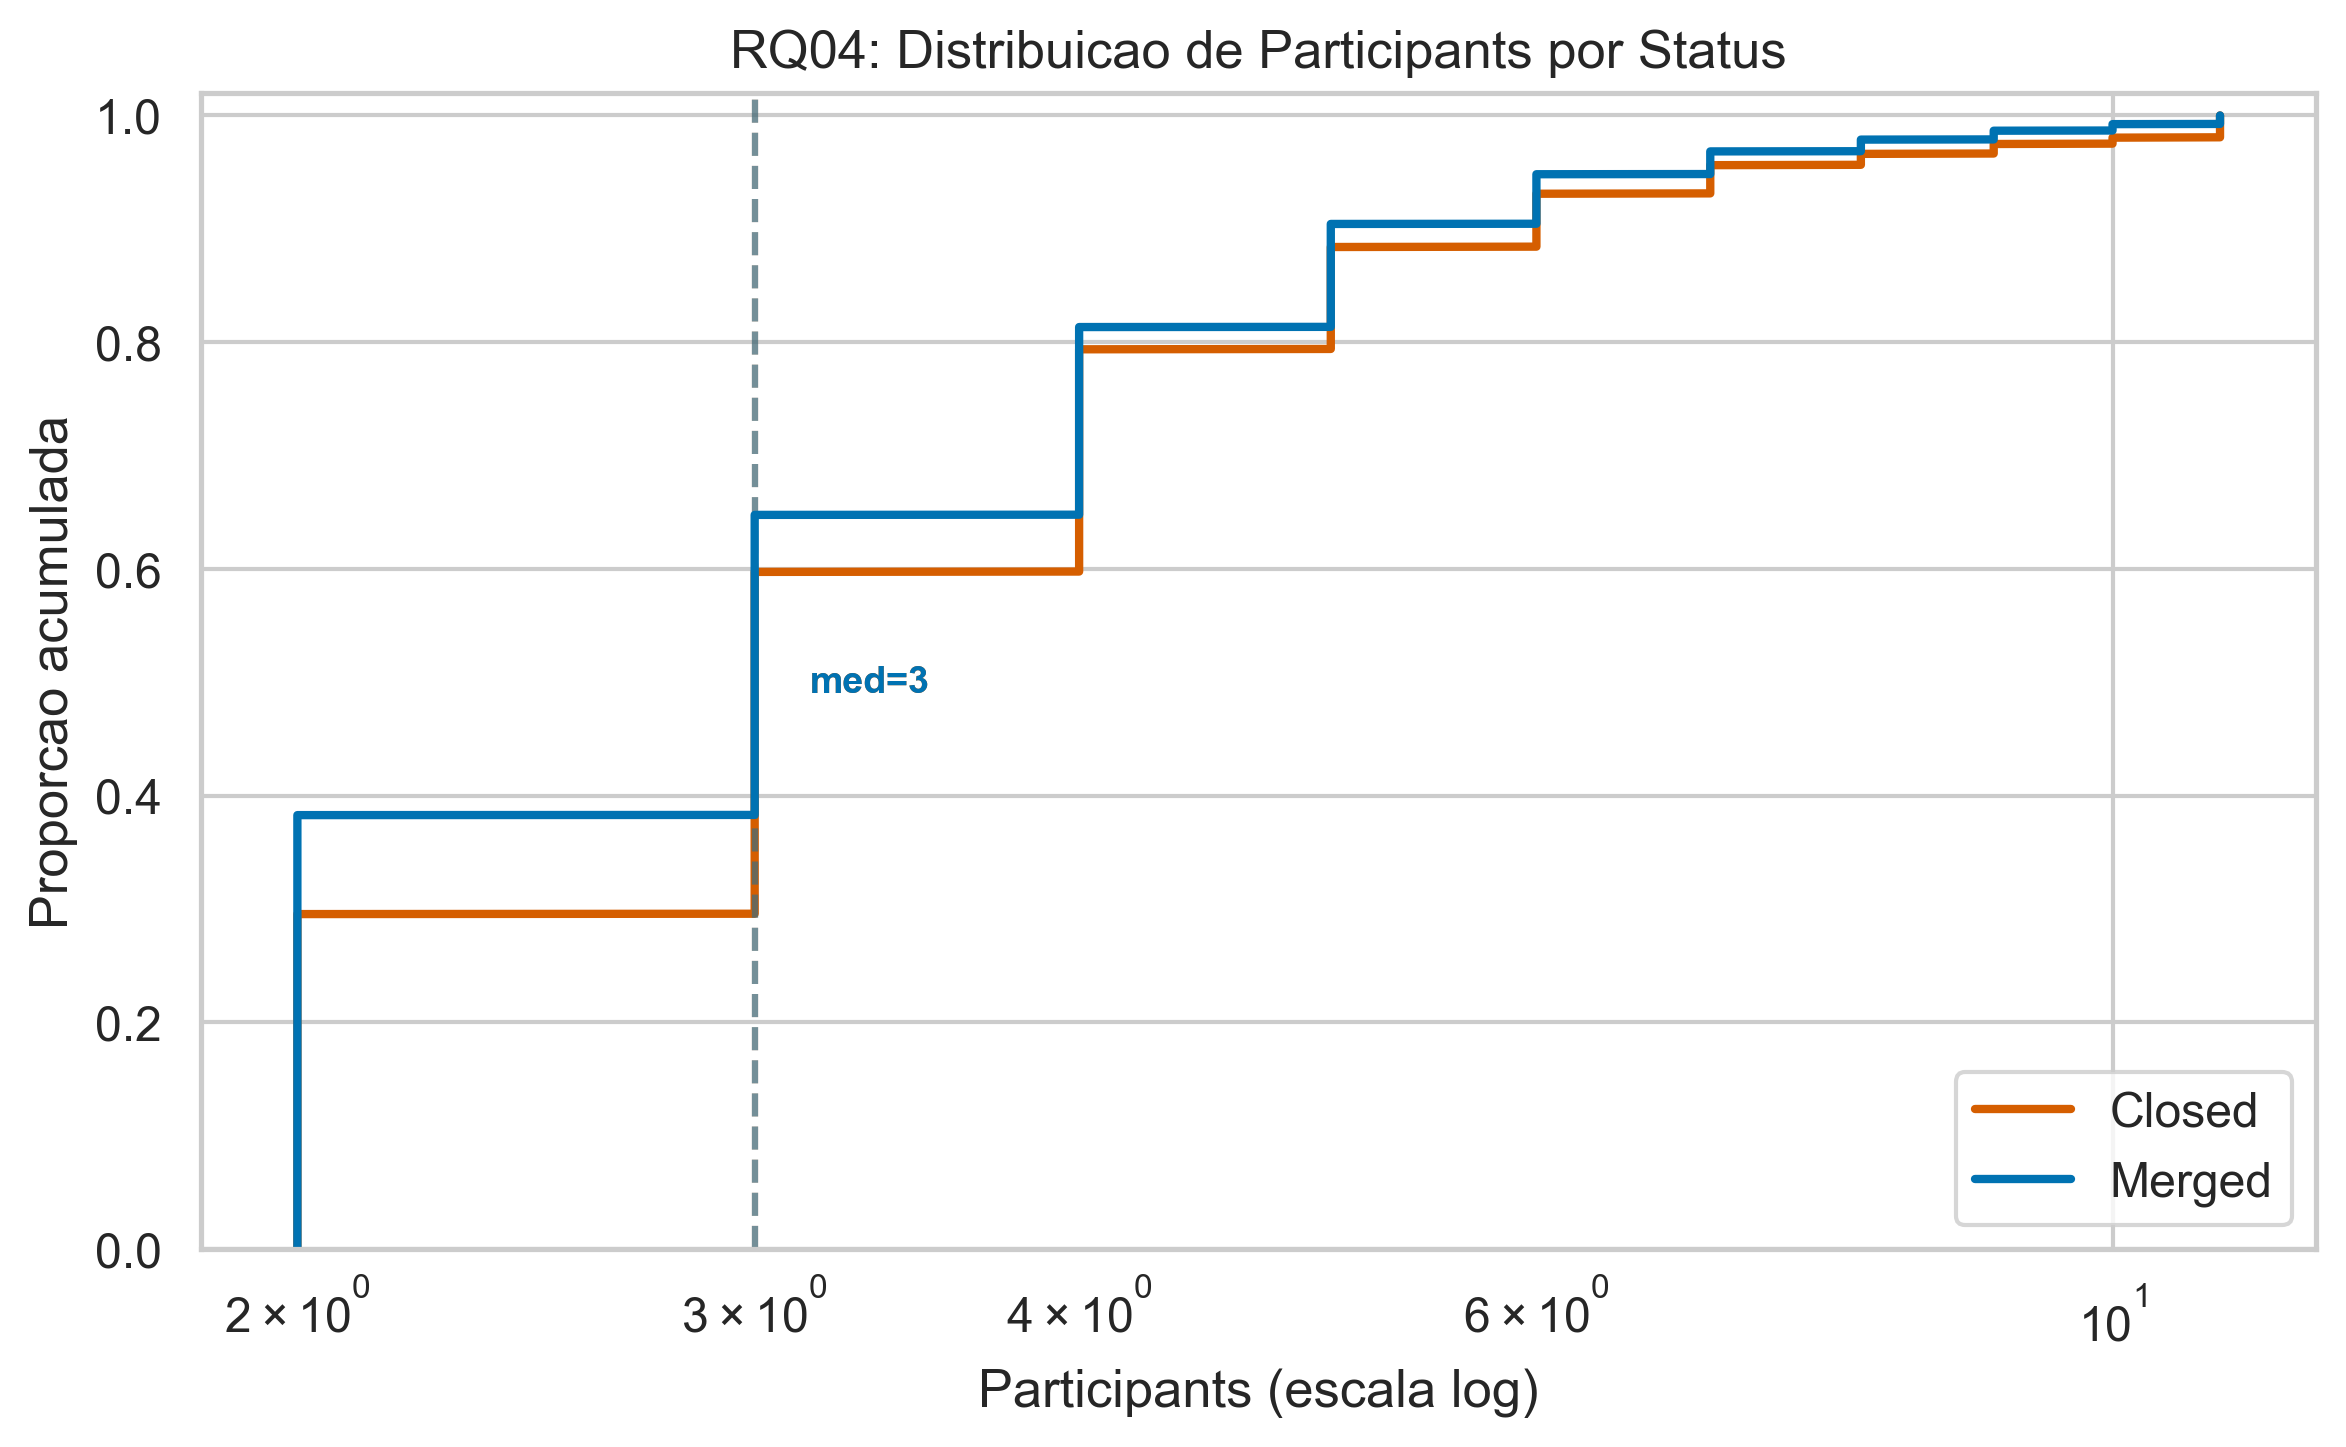
\includegraphics[width=0.85\textwidth]{figures/rq04.png}
    \caption{RQ04: ECDF do número de participantes por status de merge.}
    \label{fig:rq04}
\end{figure}

\subsection{Dimensão B: Número de Revisões}

\subsubsection{RQ05 -- Tamanho vs. Revisões}
Correlação moderada e positiva ($\rho = 0,3114$, $p < 0,0001$).
PRs maiores recebem mais revisões: mediana de 14 linhas (1 revisão)
cresce para 342 (10 revisões).

\begin{figure}[H]
    \centering
    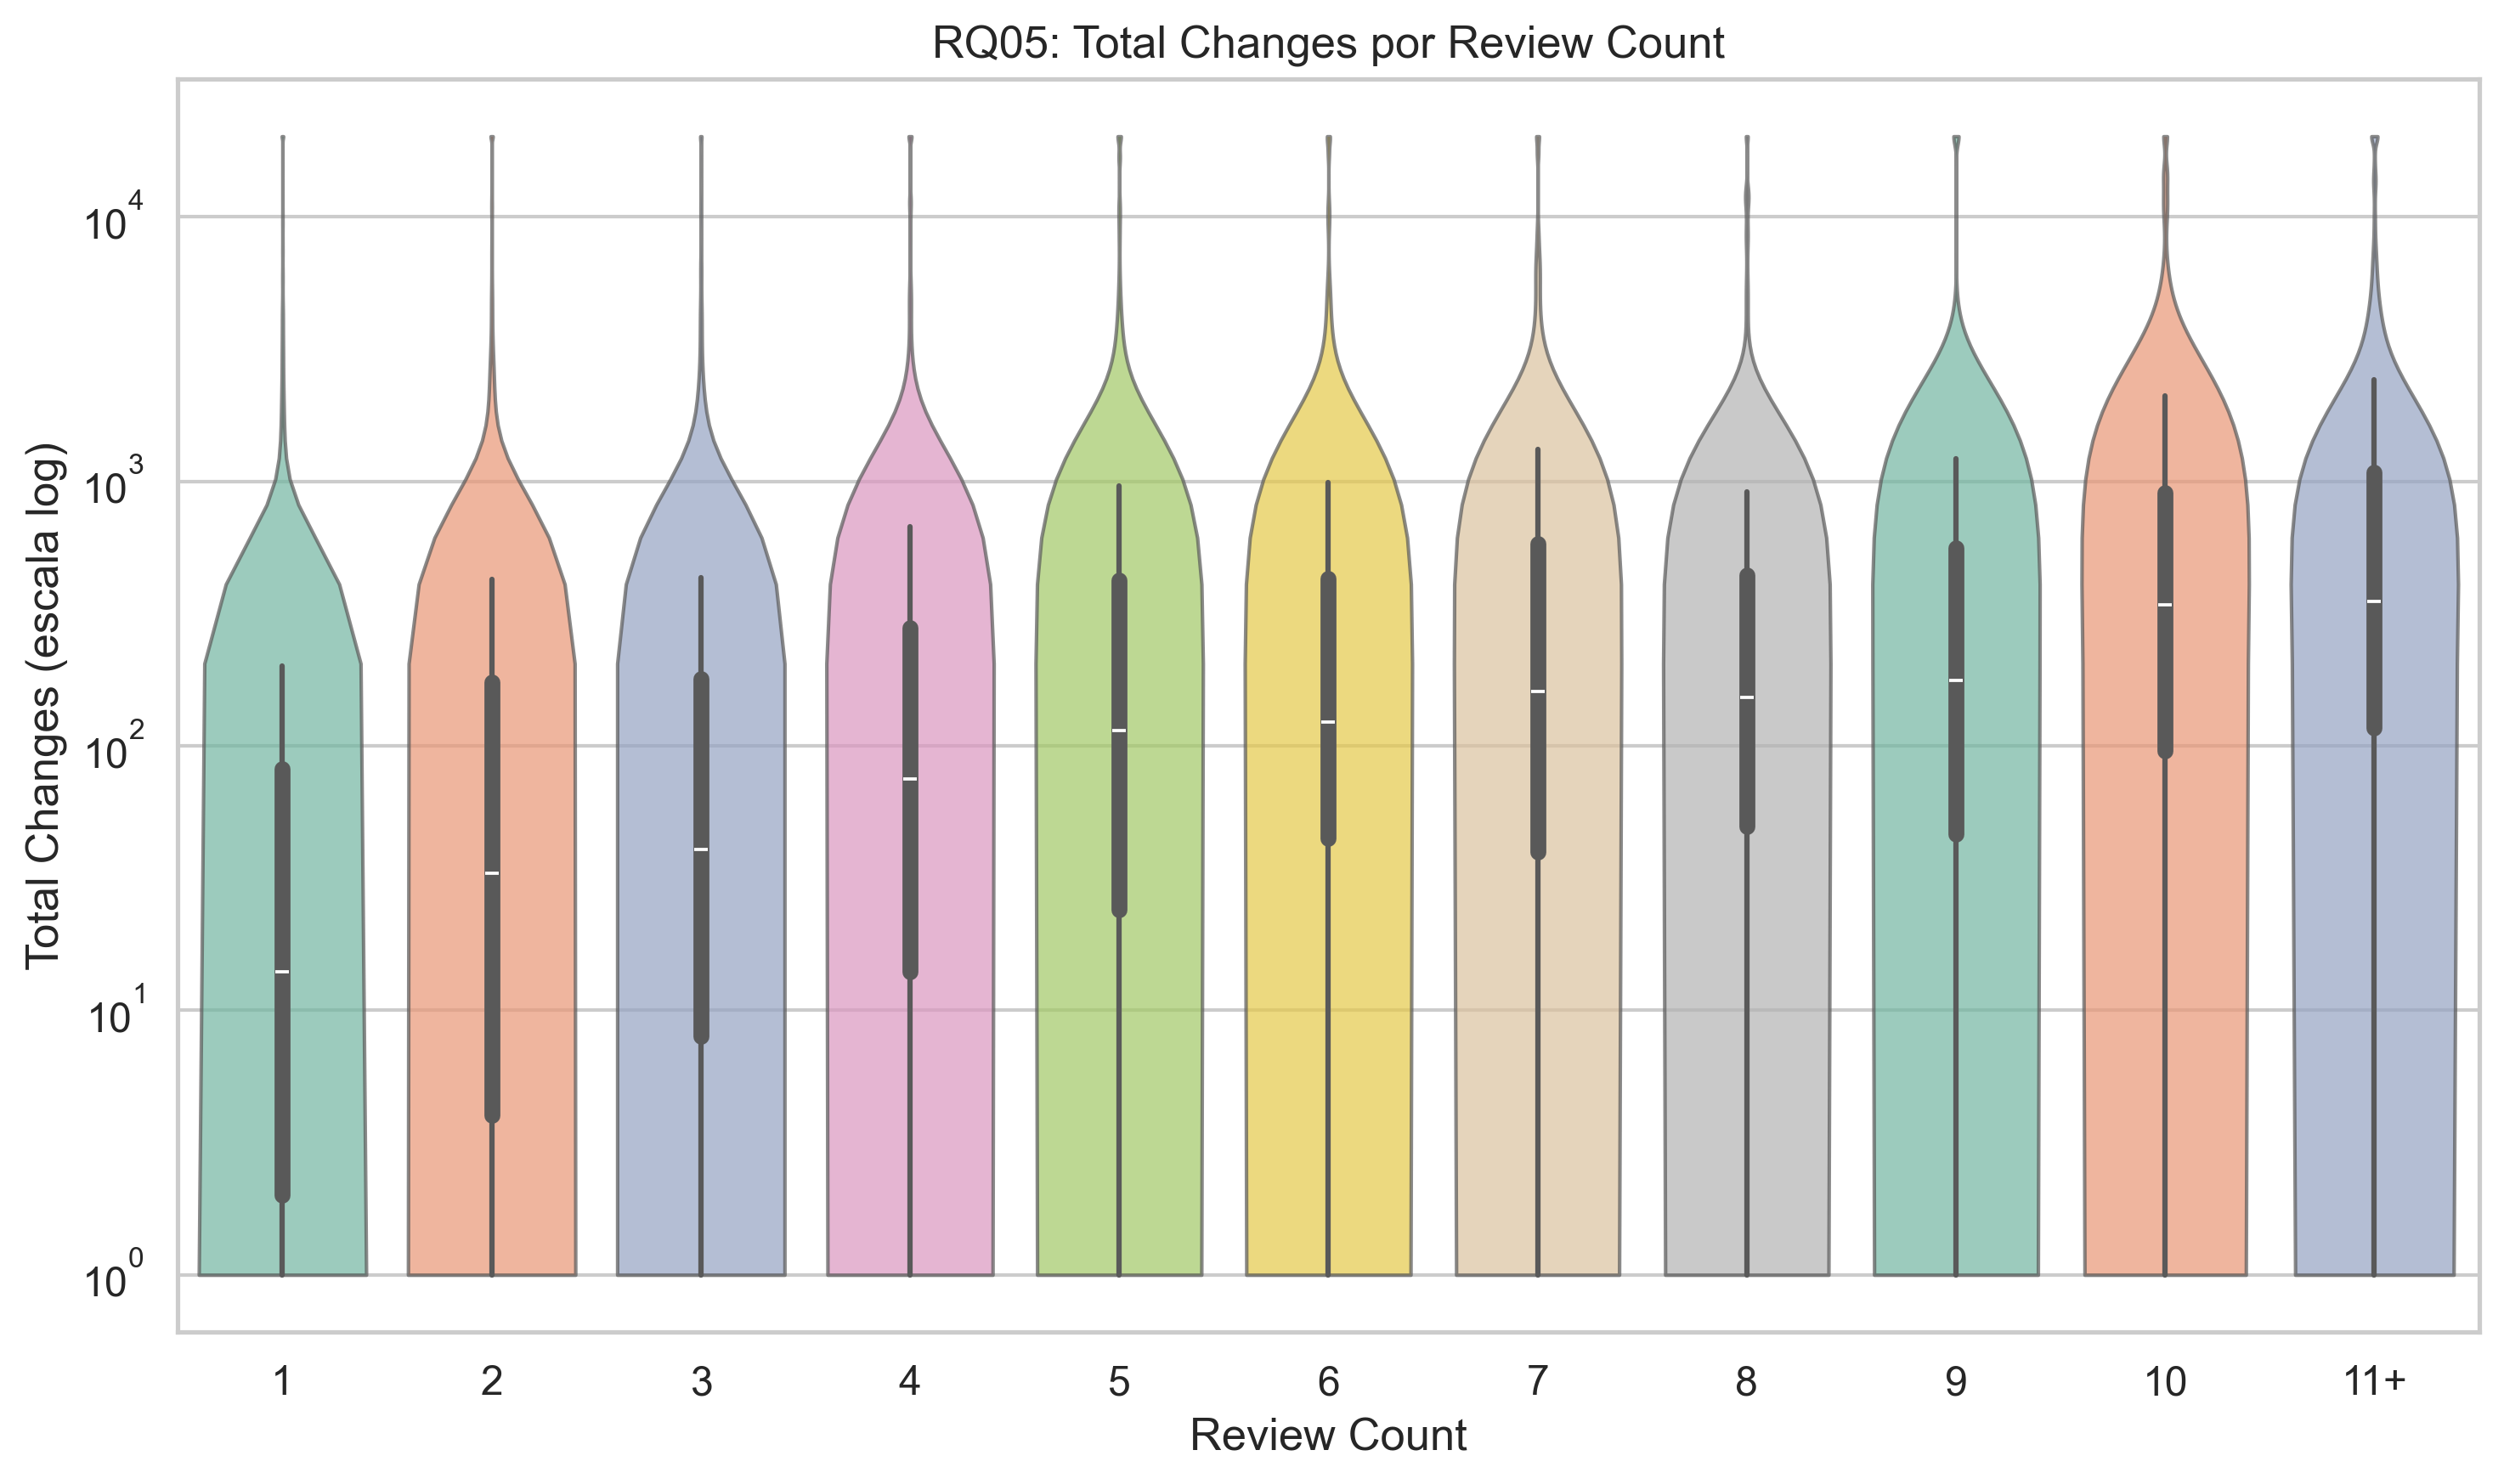
\includegraphics[width=0.85\textwidth]{figures/rq05.png}
    \caption{RQ05: Violin plot de tamanho do PR por número de revisões.}
    \label{fig:rq05}
\end{figure}

\subsubsection{RQ06 -- Tempo vs. Revisões}
Correlação desprezível ($\rho = 0,0917$, $p < 0,0001$).
Tempo de análise não aumenta sistematicamente com número de revisões.

\begin{figure}[H]
    \centering
    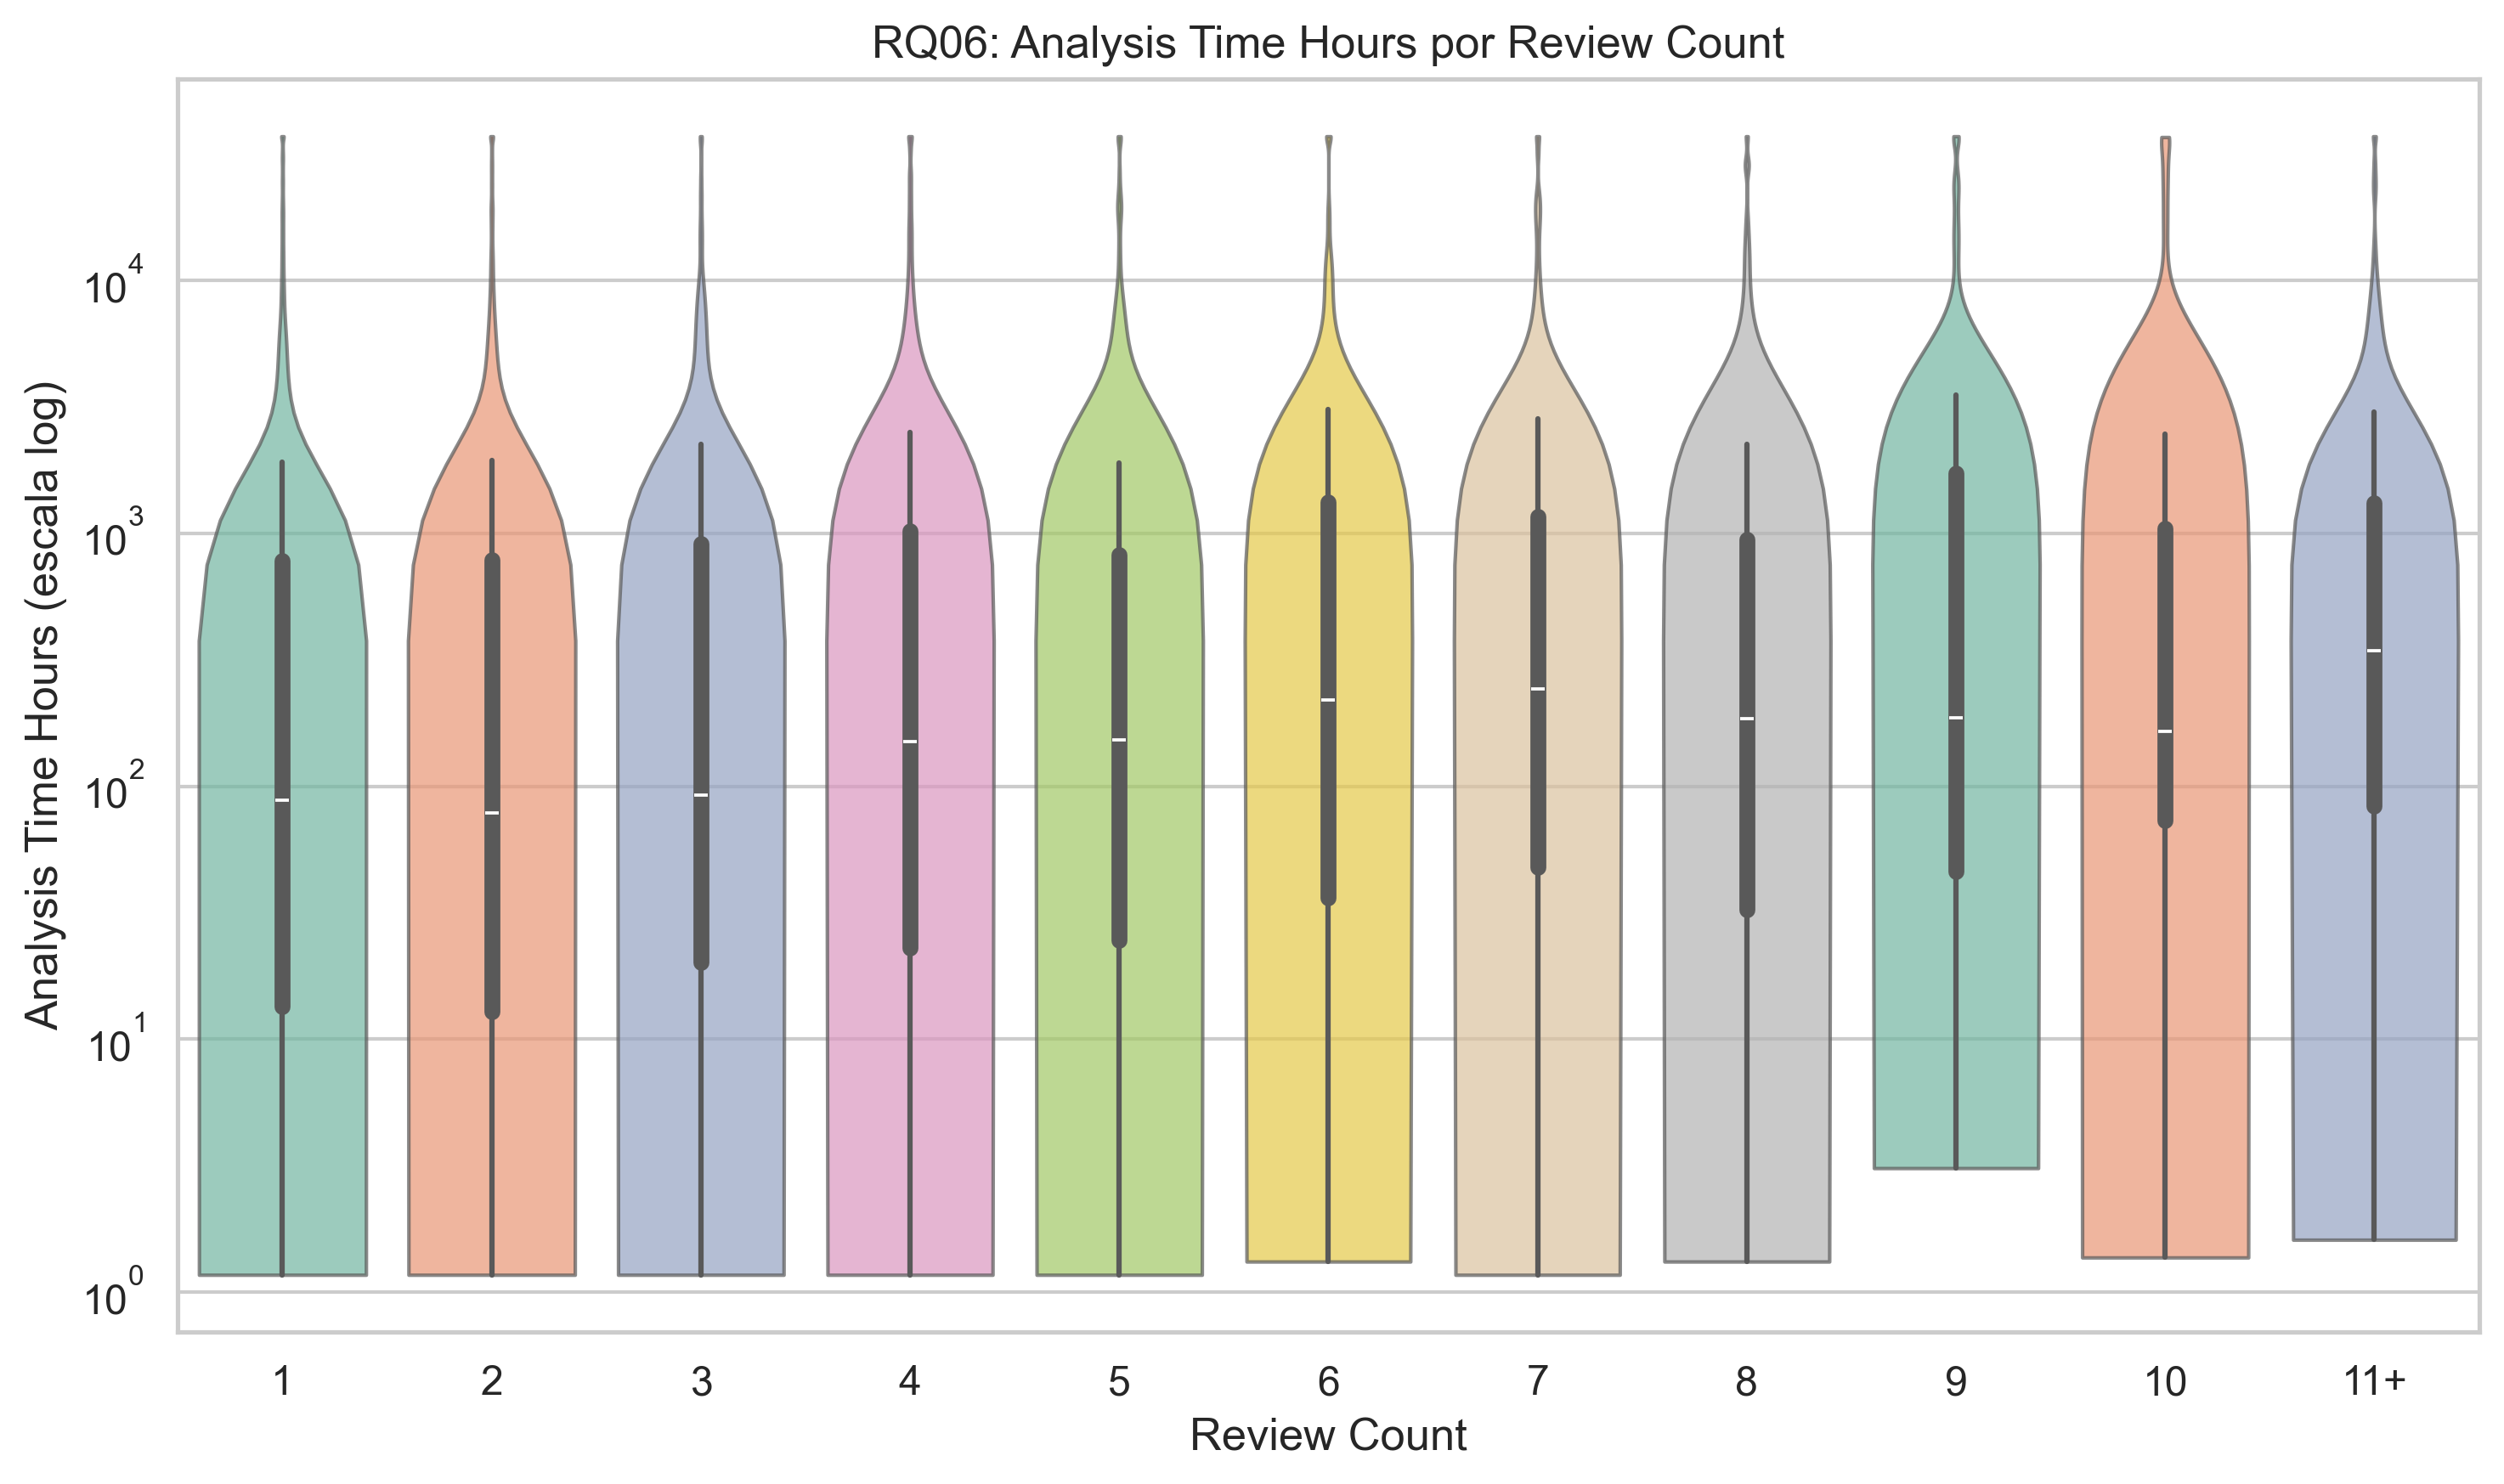
\includegraphics[width=0.85\textwidth]{figures/rq06.png}
    \caption{RQ06: Violin plot de tempo de análise por número de revisões.}
    \label{fig:rq06}
\end{figure}

\subsubsection{RQ07 -- Descrição vs. Revisões}
Correlação fraca ($\rho = 0,1861$, $p < 0,0001$).
Descrições maiores tendem a receber ligeiramente mais revisões.

\begin{figure}[H]
    \centering
    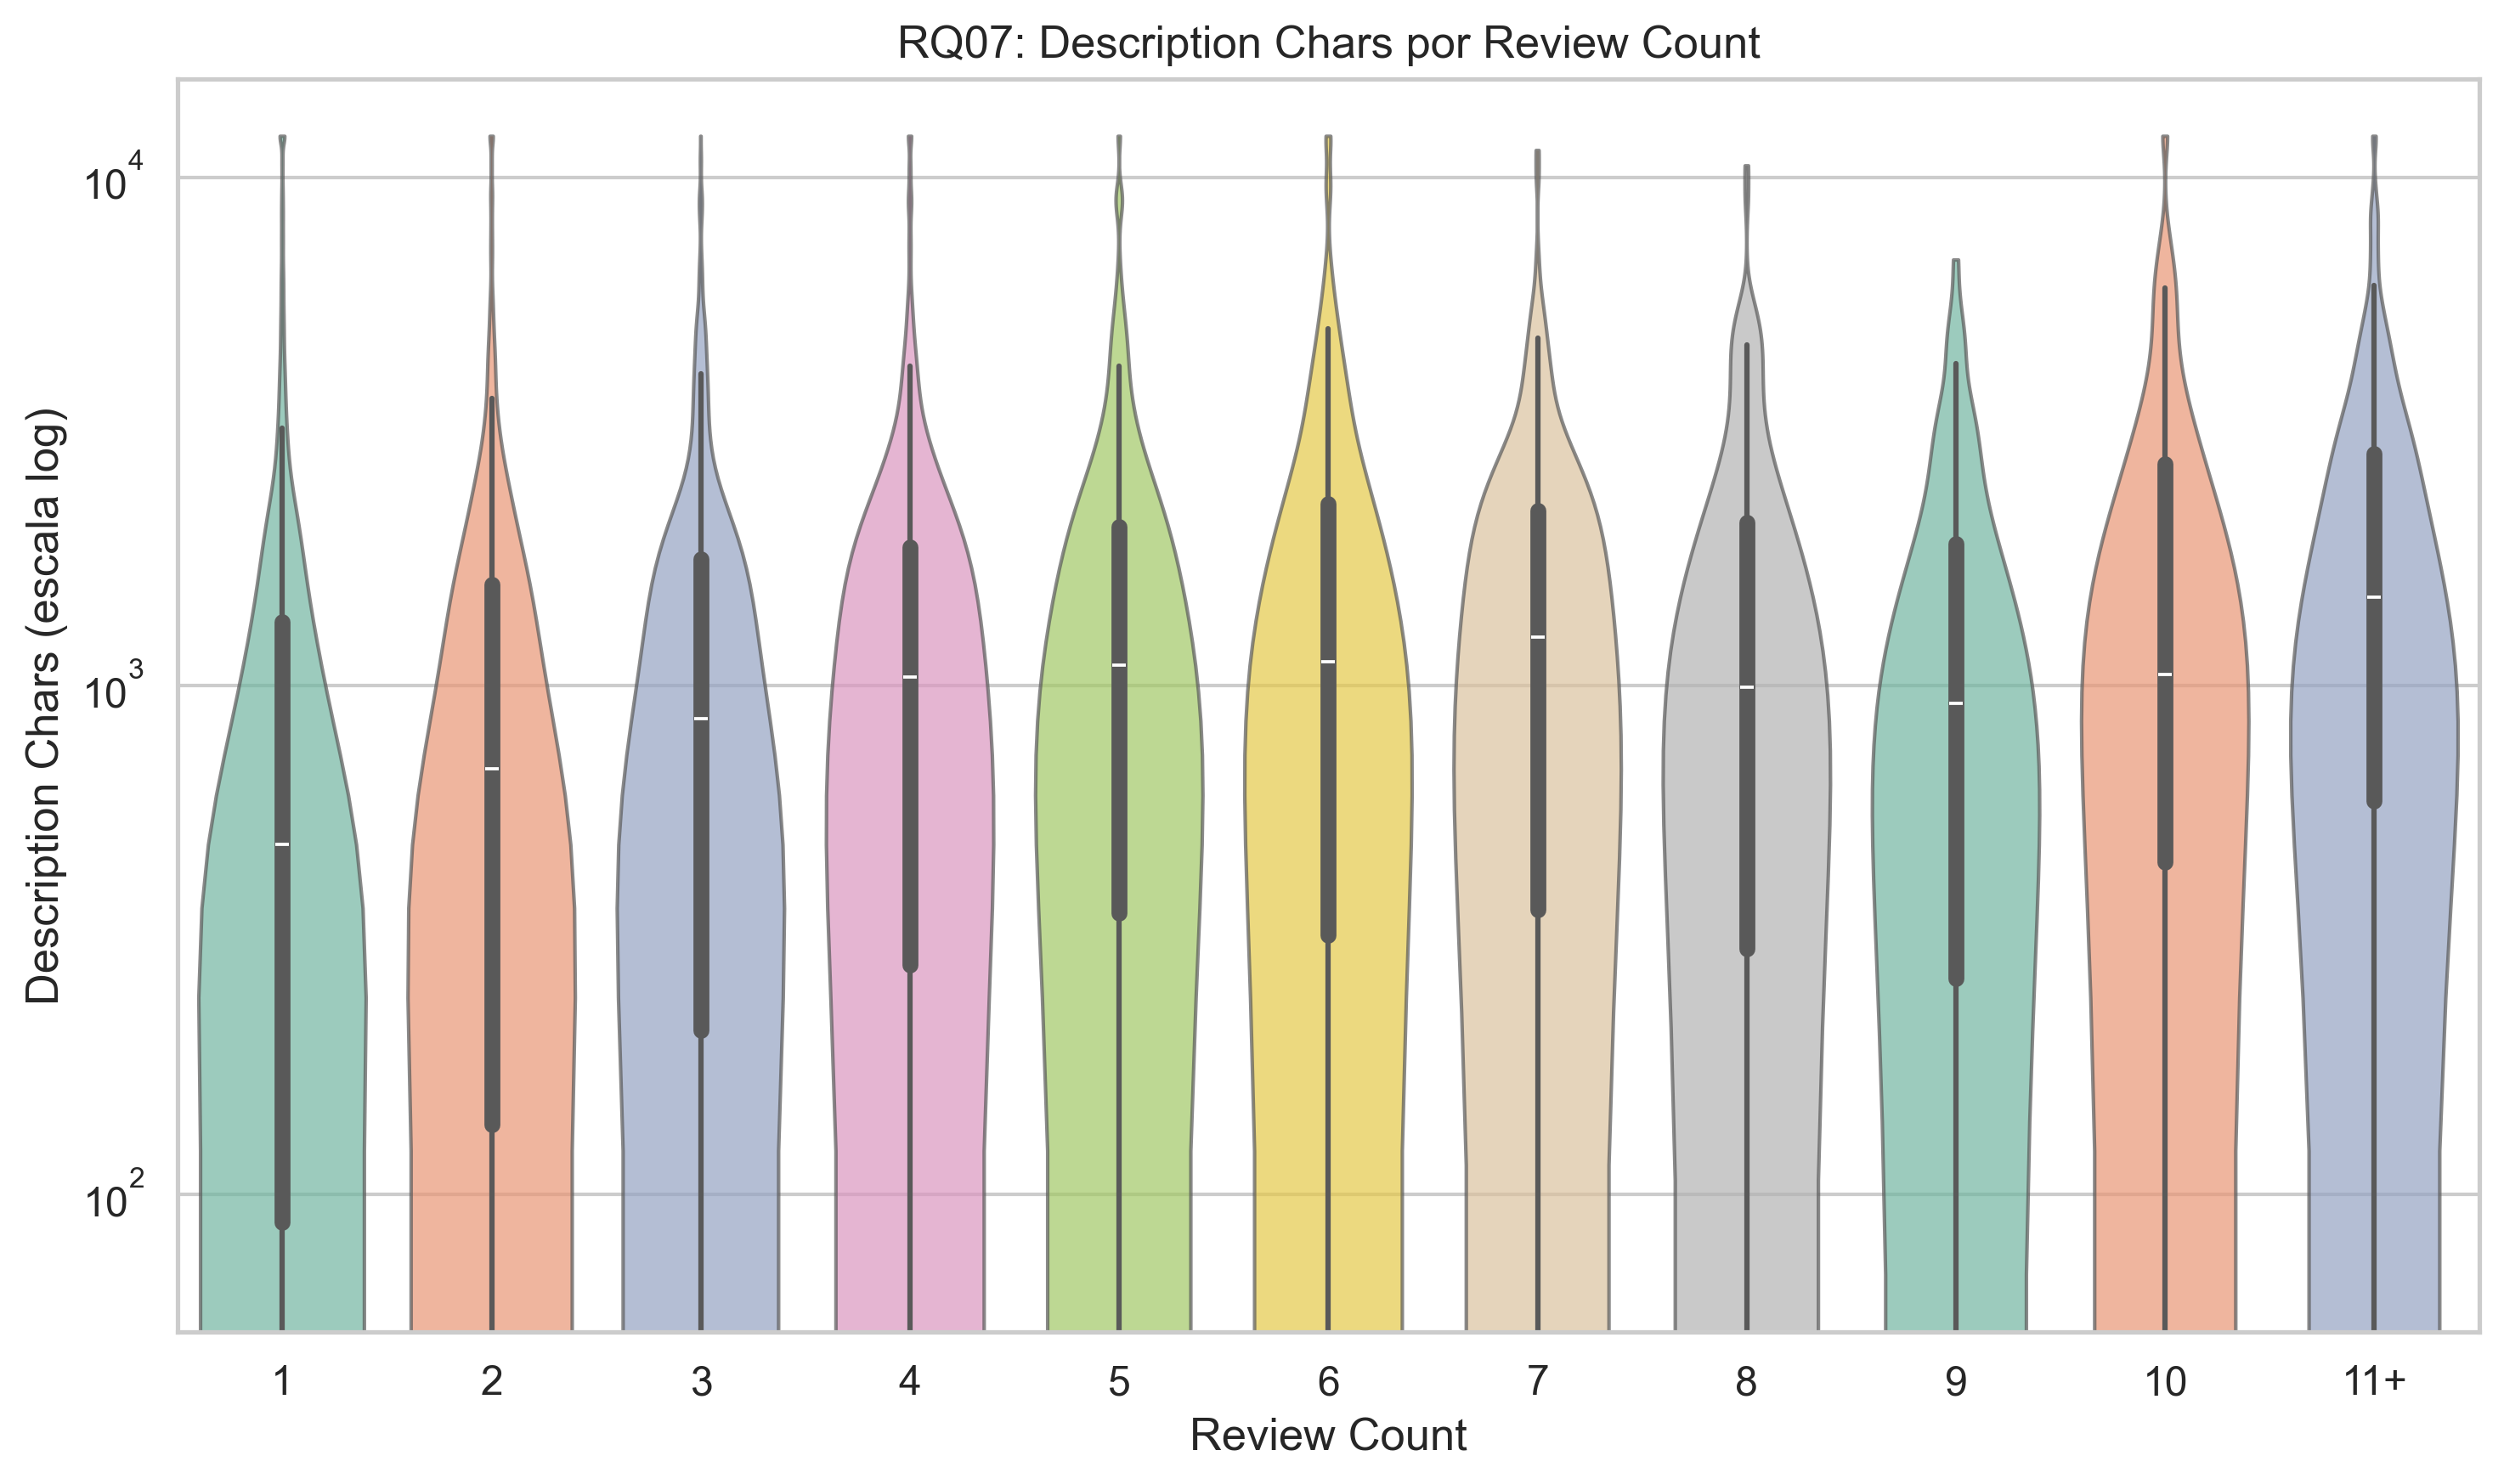
\includegraphics[width=0.85\textwidth]{figures/rq07.png}
    \caption{RQ07: Violin plot de tamanho da descrição por número de revisões.}
    \label{fig:rq07}
\end{figure}

\subsection{Matriz de Correlação}

A matriz de correlações entre todas as métricas revela a forte correlação
entre \texttt{lines\_added} e \texttt{total\_changes} ($\rho = 0,97$),
confirmando que são medidas redundantes.

\begin{figure}[H]
    \centering
    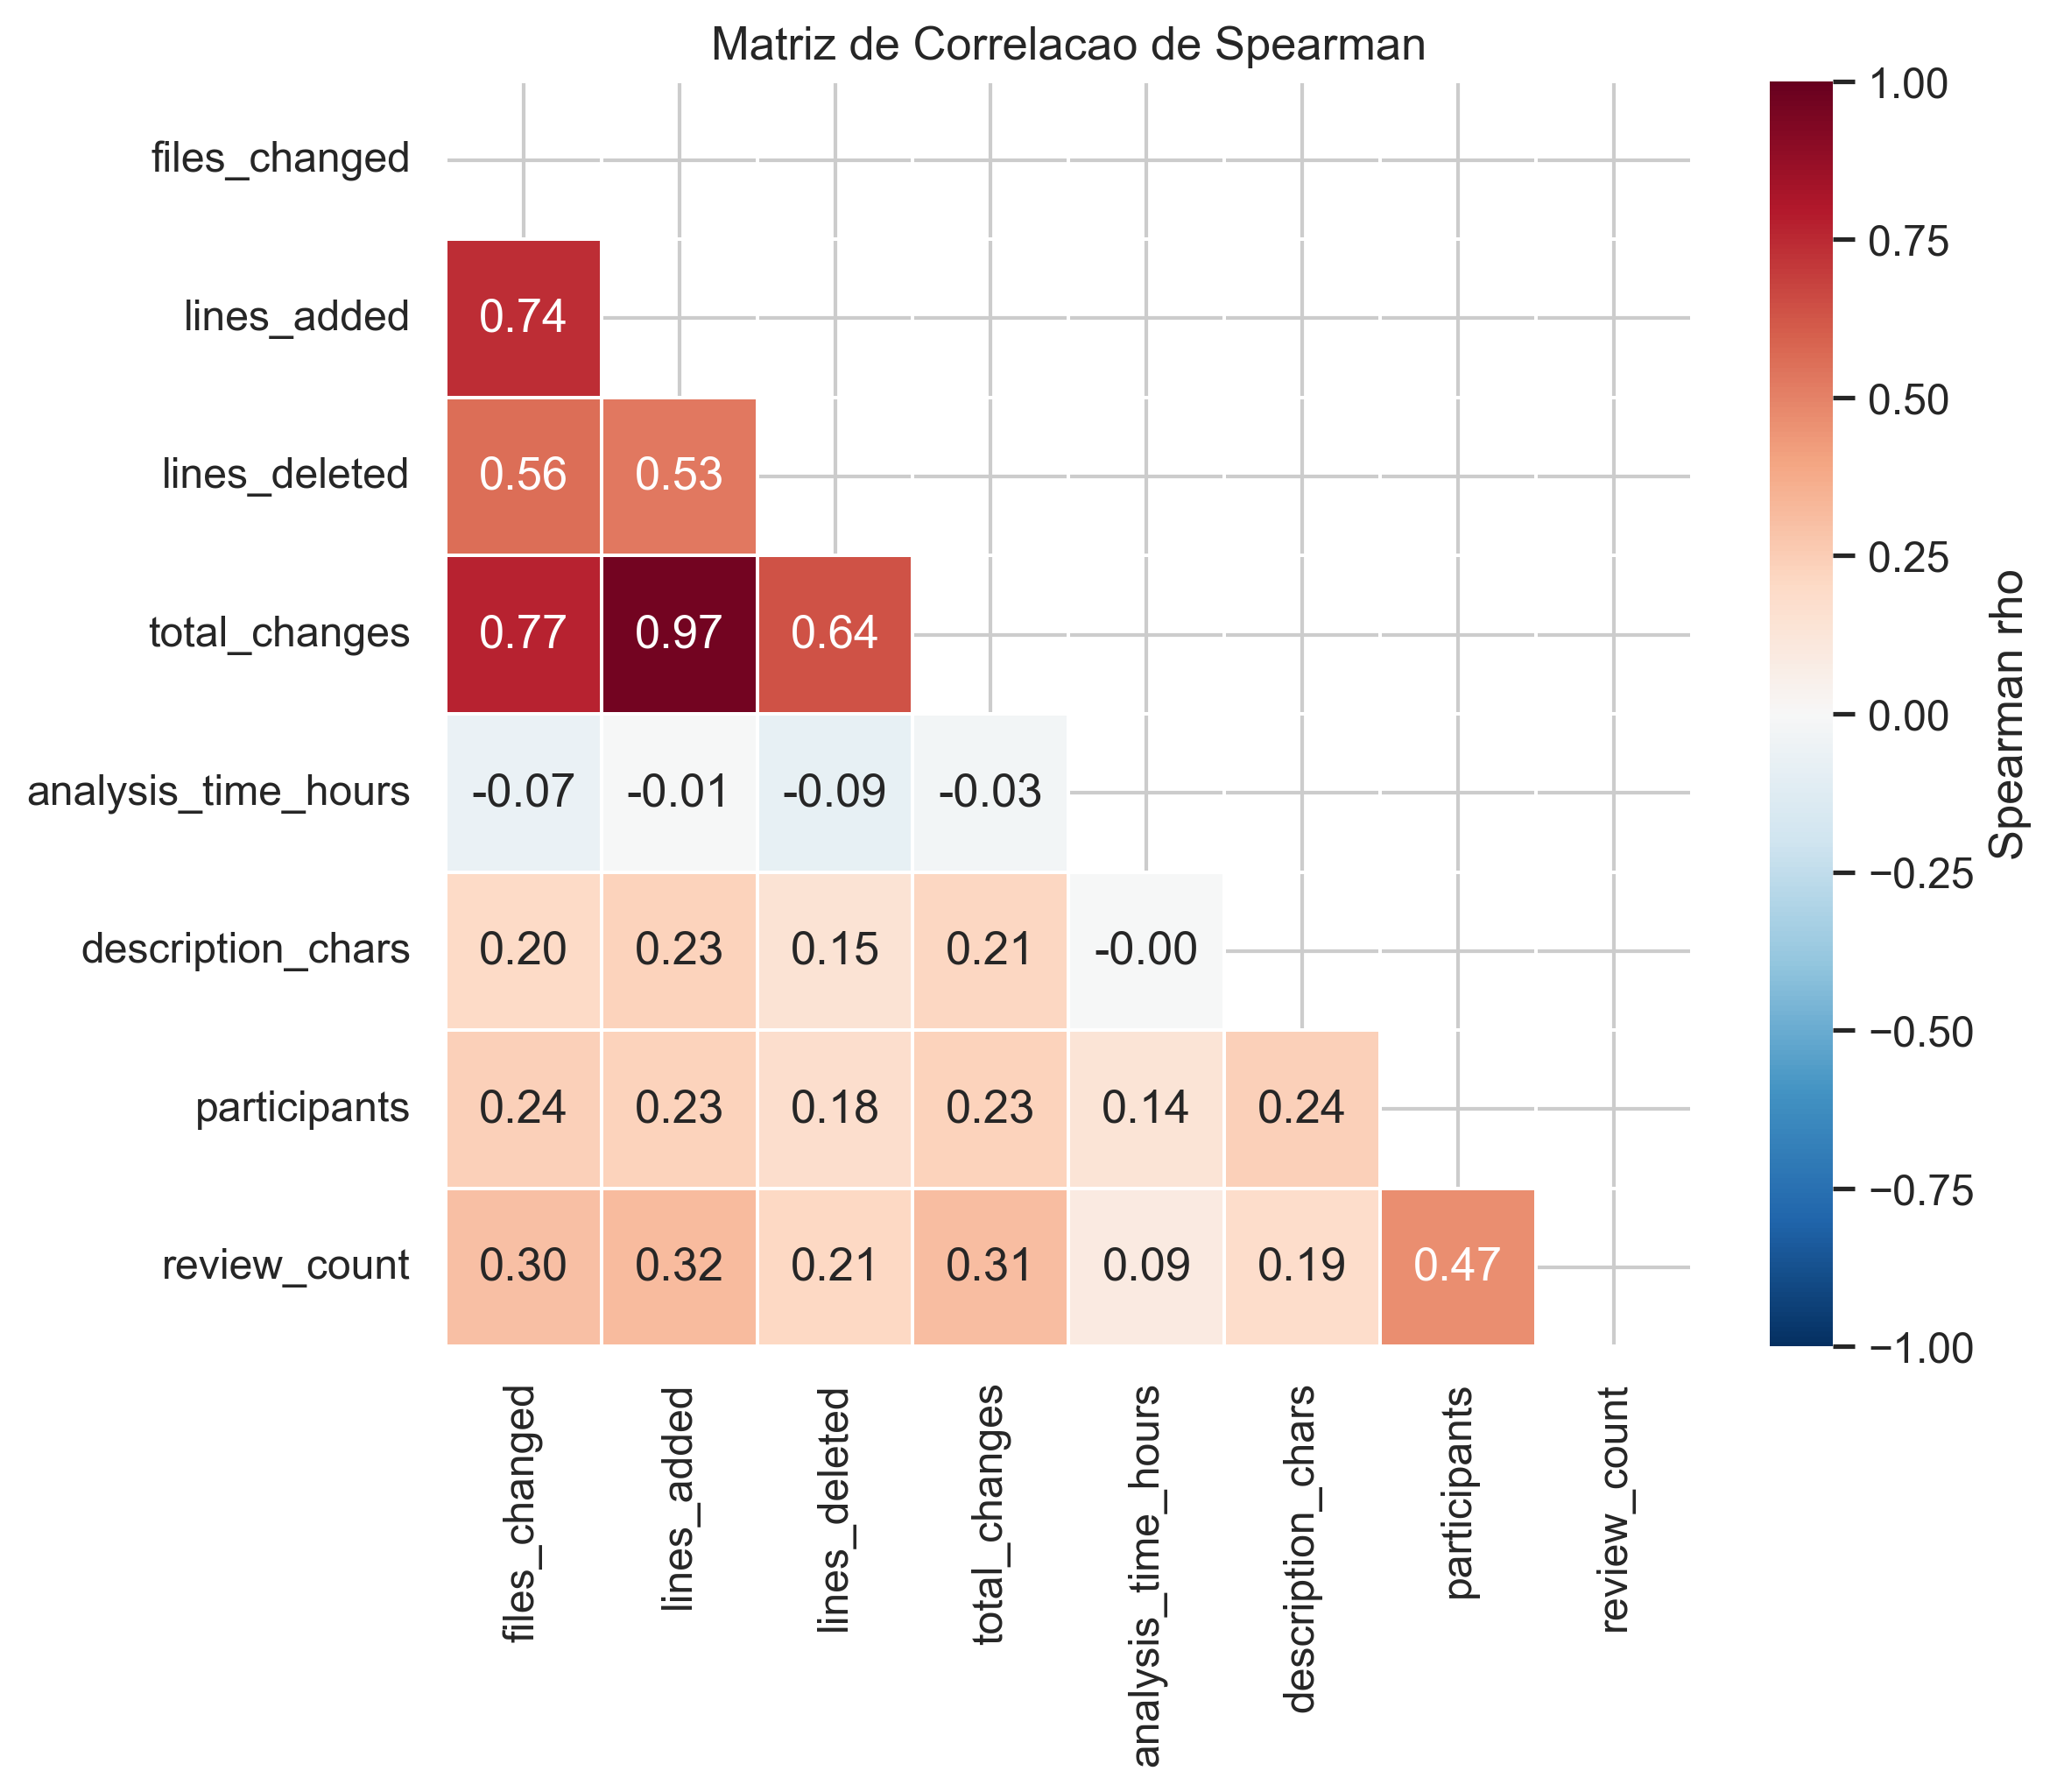
\includegraphics[width=\textwidth]{figures/correlation_matrix.png}
    \caption{Matriz de correlação de Spearman entre todas as métricas.}
    \label{fig:corr}
\end{figure}

\subsection{Distribuições Gerais}

As distribuições de todas as métricas por status de merge, apresentadas
em ECDF, mostram que a diferença mais marcante está no tempo de análise.

\begin{figure}[H]
    \centering
    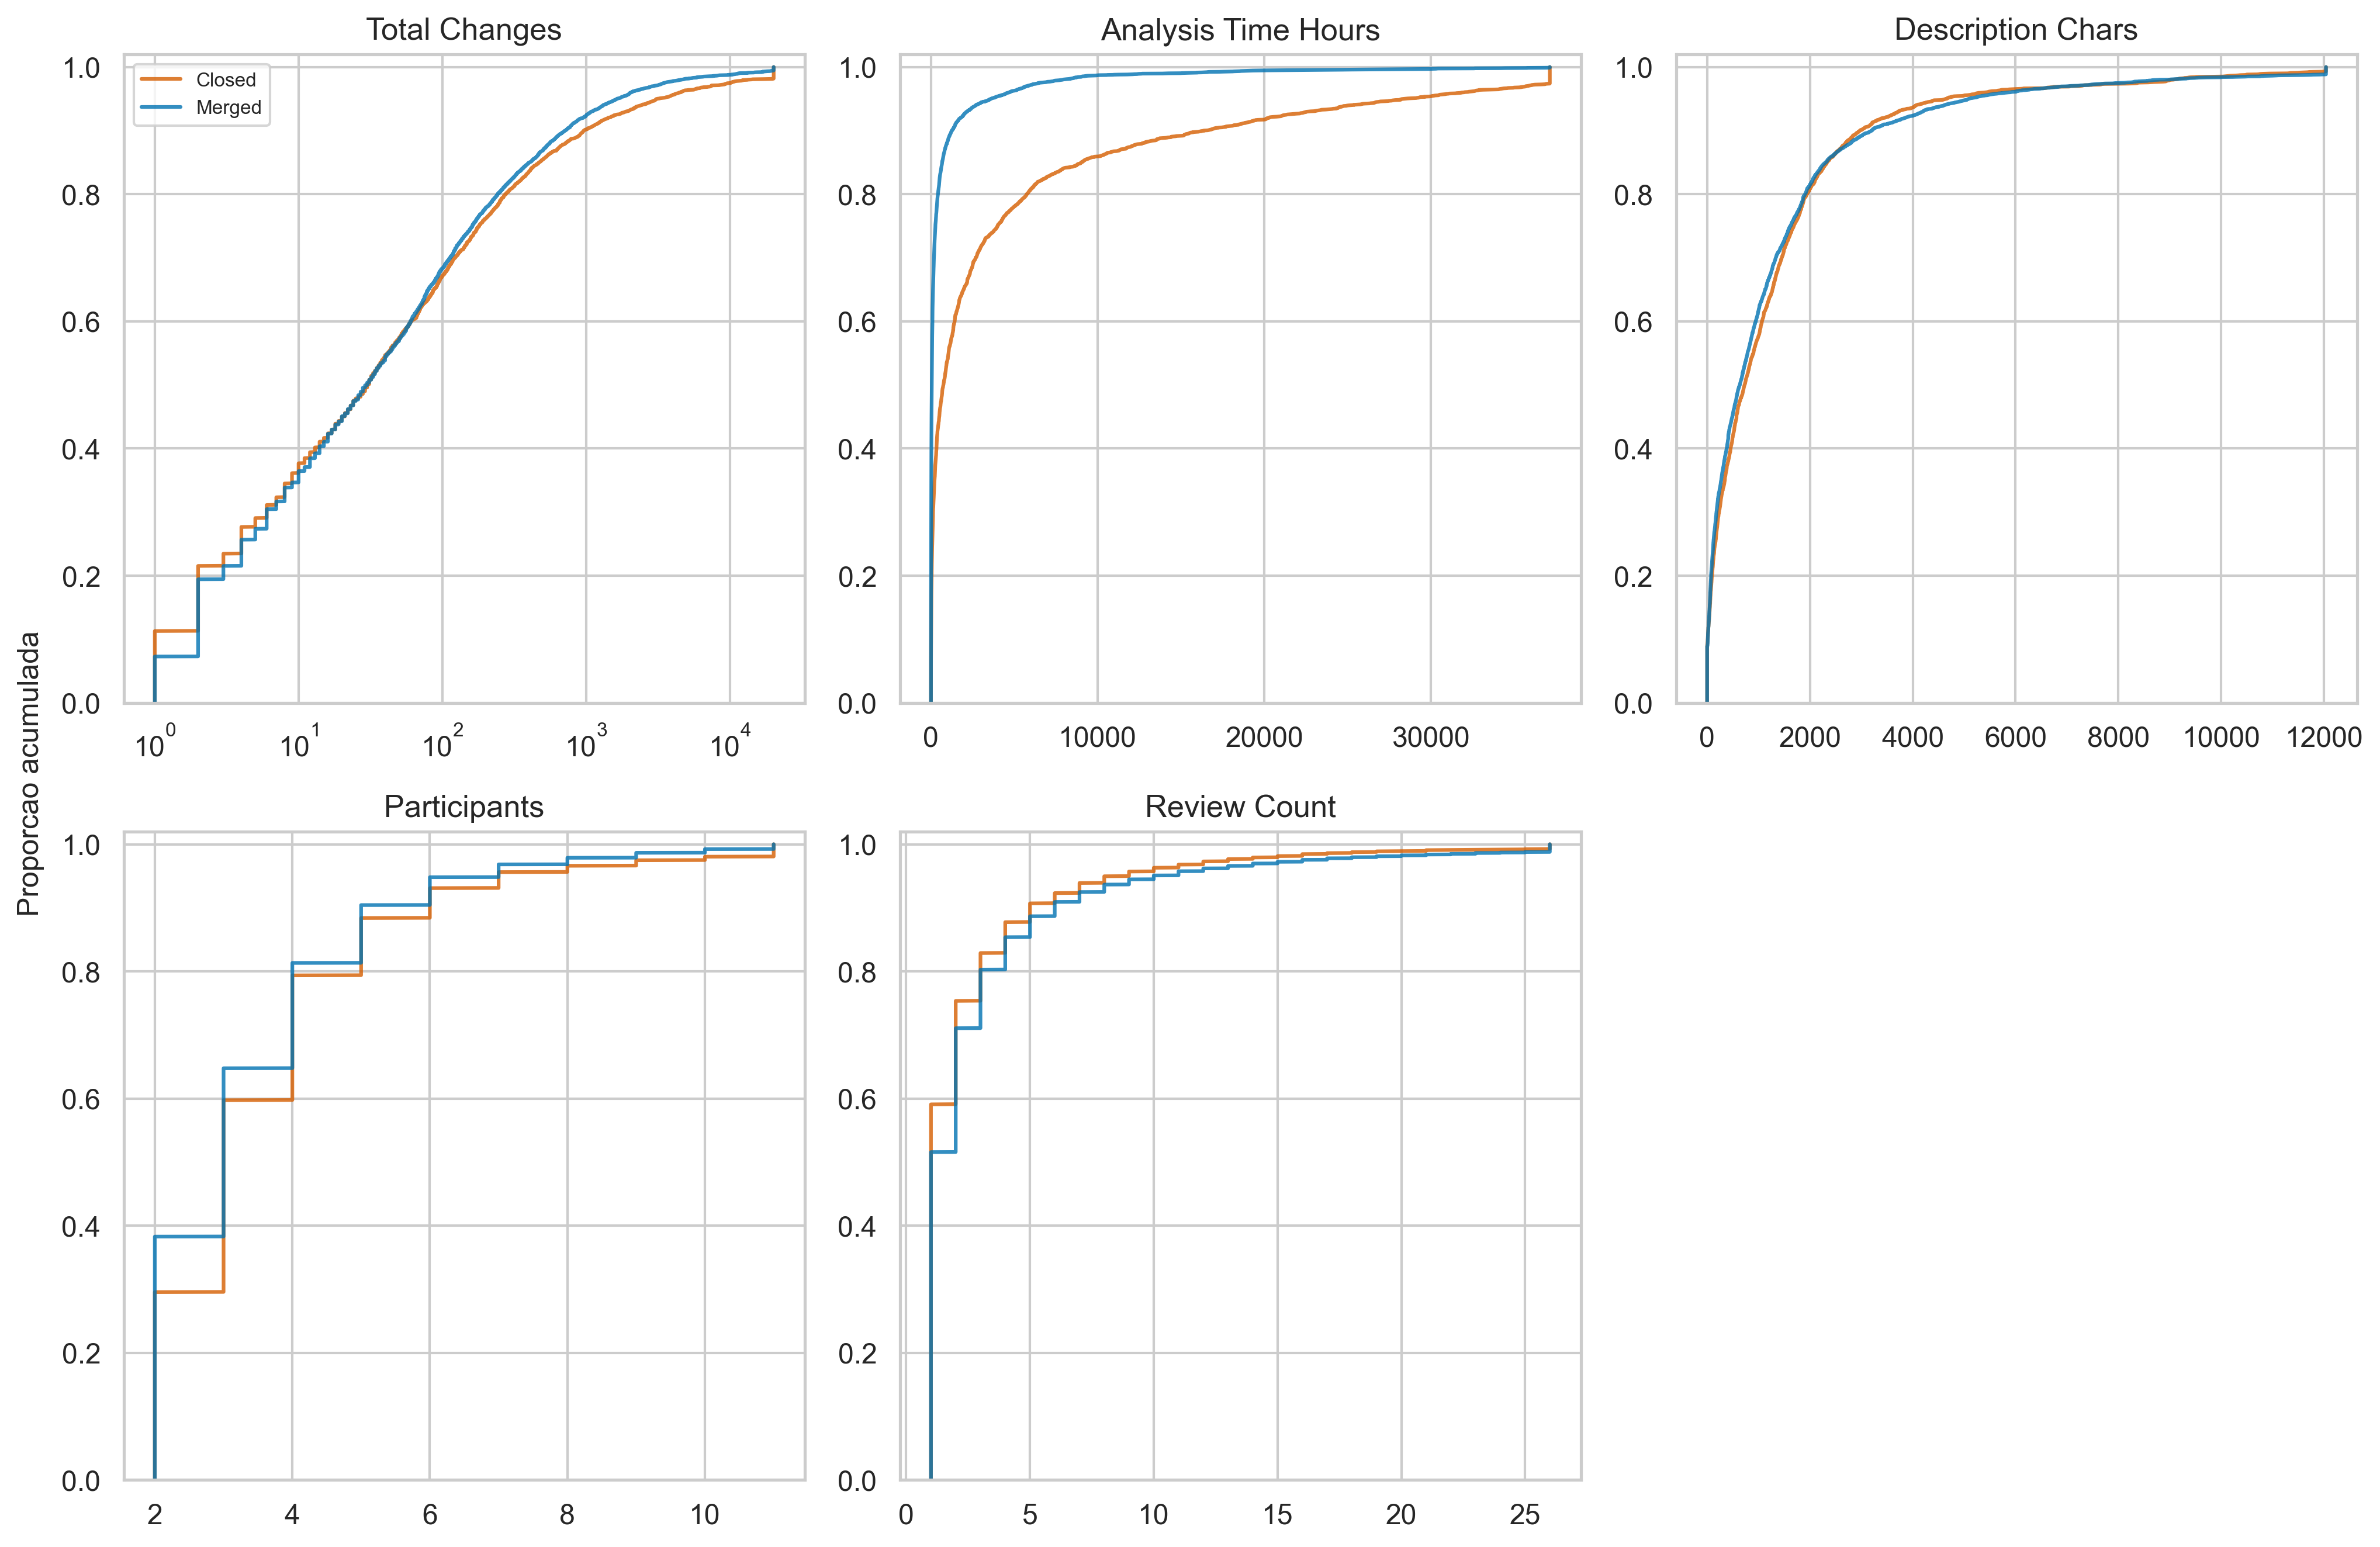
\includegraphics[width=\textwidth]{figures/distribution_ecdf.png}
    \caption{ECDF de todas as métricas por status de merge.}
    \label{fig:ecdf}
\end{figure}

\subsection{Revisões por Status}

PRs merged tendem a ter mediana de 1 revisão, enquanto closed têm mediana de 2.

\begin{figure}[H]
    \centering
    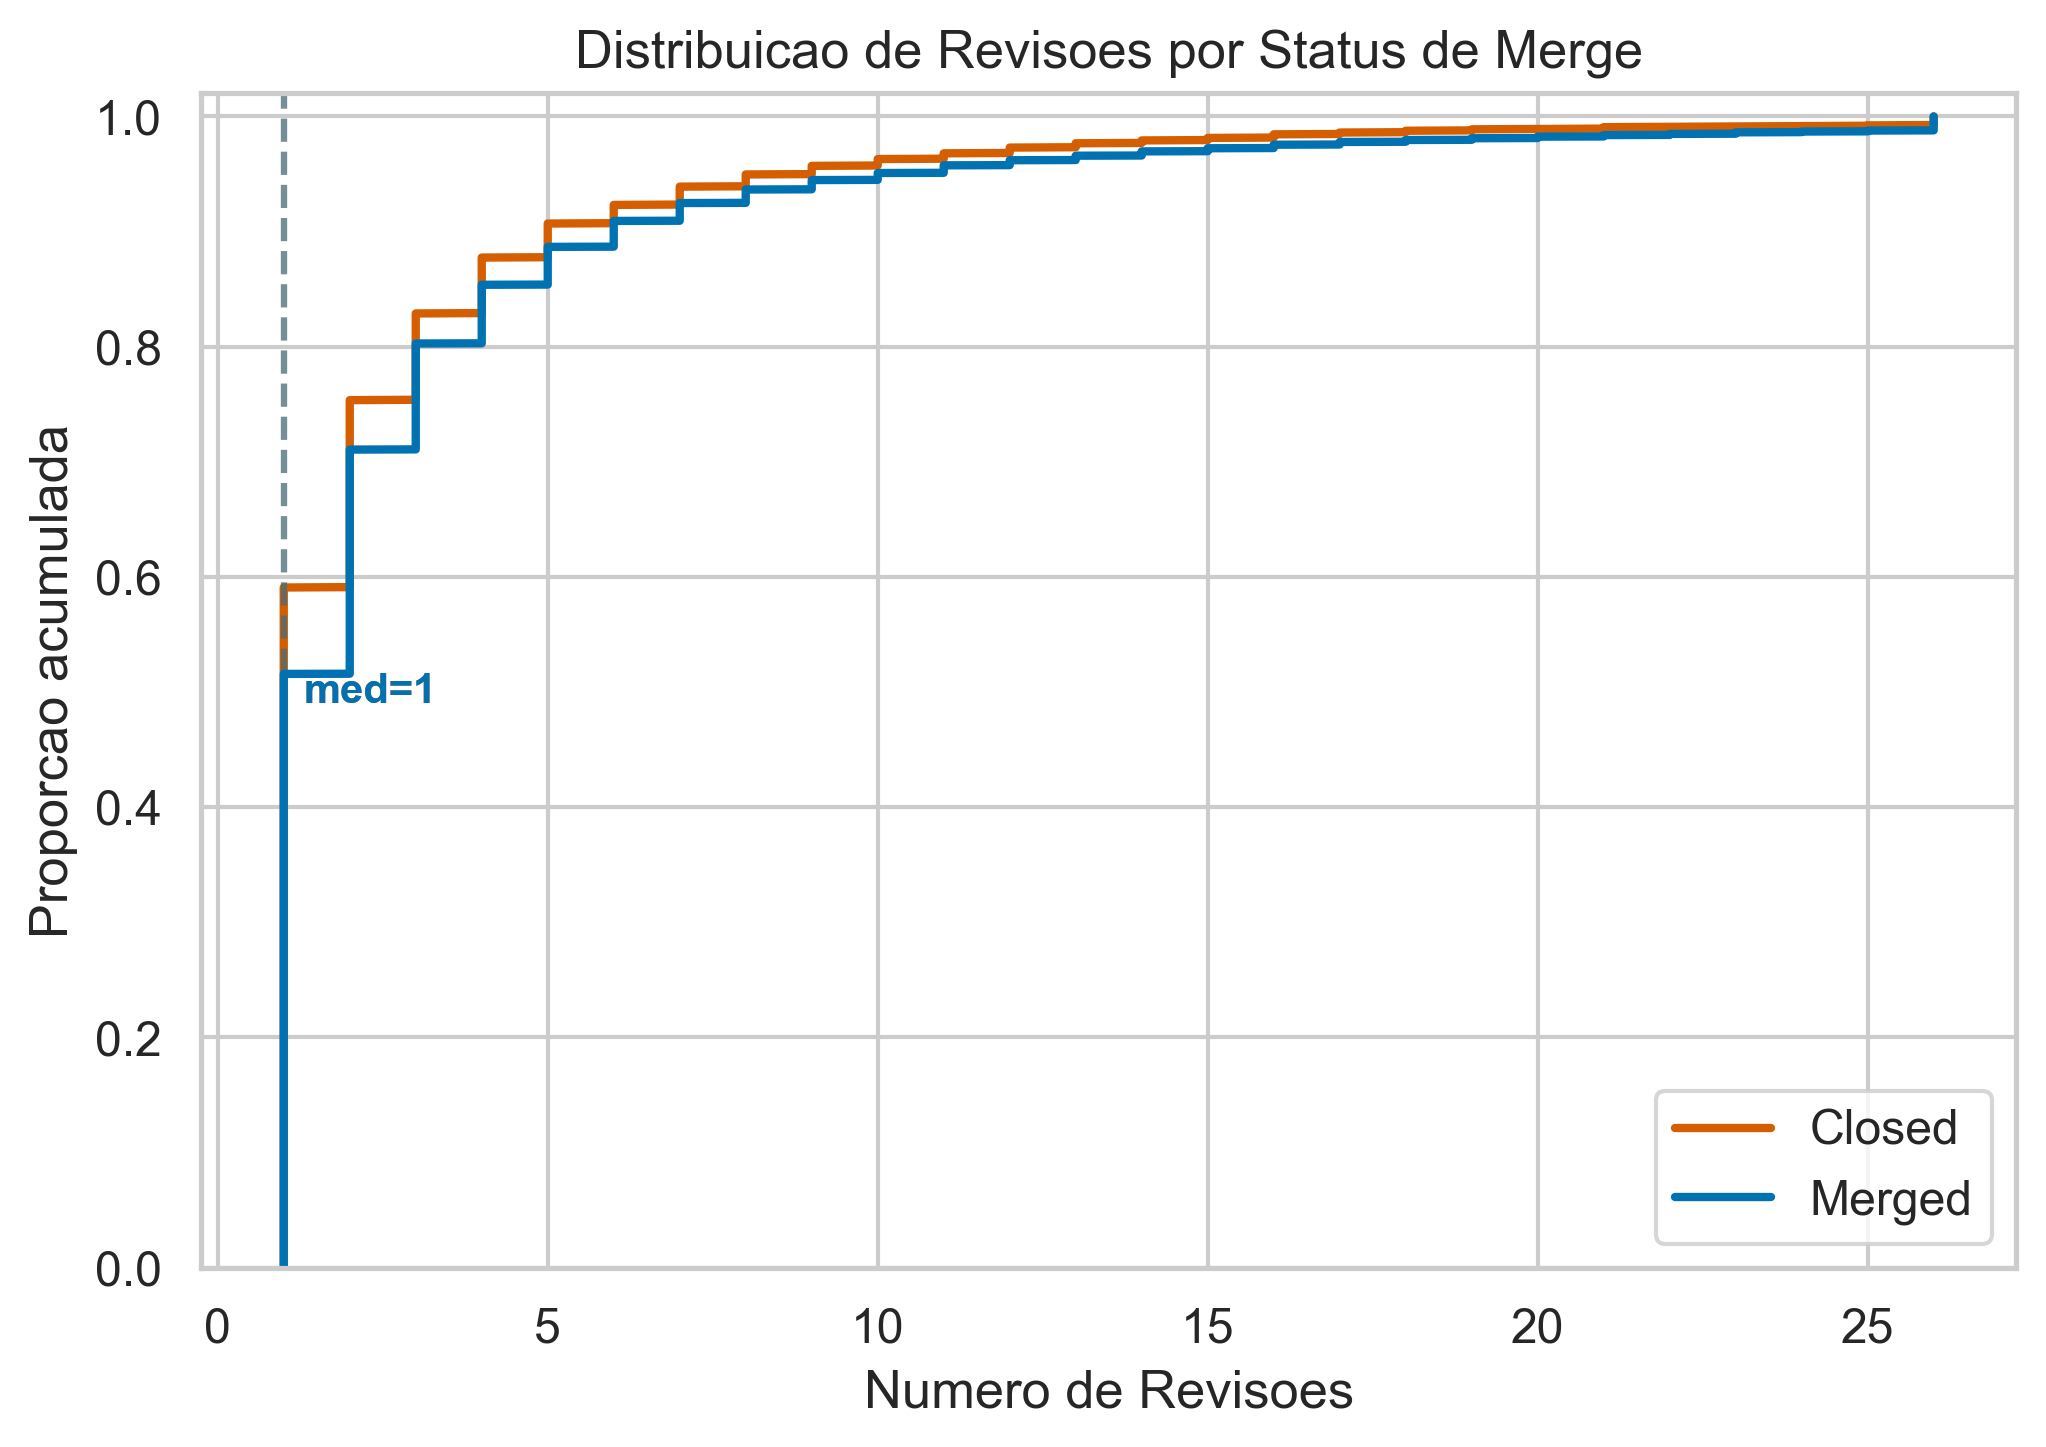
\includegraphics[width=0.85\textwidth]{figures/merged_vs_reviews.png}
    \caption{ECDF do número de revisões por status de merge.}
    \label{fig:reviews}
\end{figure}


\section{Discussão}
Os resultados revelam padrões importantes sobre code review em repositórios
populares do GitHub.

\textbf{Dimensão A -- Status do PR:}
O tempo de análise é o único fator com correlação moderada ao status de merge
(RQ02, $\rho = -0,3910$). Isso sugere que PRs que são integrados rapidamente
têm maior chance de merge. Possíveis explicações incluem: PRs simples e bem
preparados passam mais rápido pela revisão, ou PRs que demoram muito perdem
relevância ou conflitam com mudanças mais recentes.

As demais métricas (tamanho, descrição, participantes) apresentam correlações
desprezíveis com o status.

\textbf{Dimensão B -- Número de Revisões:}
O tamanho do PR (RQ05, $\rho = 0,3114$) mostra correlação moderada com o
número de revisões. PRs maiores demandam mais atenção de revisores, como
evidenciado pelo crescimento da mediana de alterações de 14 (1 revisão)
para 342 (10 revisões). O tempo de análise (RQ06, $\rho = 0,0917$) e
o tamanho da descrição (RQ07, $\rho = 0,1861$) apresentam correlações
desprezíveis e fracas, respectivamente.

\textbf{Limitações:}
Os campos de comentários não foram corretamente coletados, limitando nossa
análise de ``interações'' ao número de participantes. Além disso, a amostra
compreende apenas repositórios populares, o que pode não refletir projetos
menores ou corporativos. A winsorização no percentil 99, embora necessária
para mitigar outliers extremos, pode ter removido informações relevantes
sobre PRs excepcionalmente grandes.


\section{Conclusão}
Este estudo analisou 9.075 Pull Requests de 197 repositórios populares do GitHub,
investigando fatores que influenciam o merge e o número de revisões.

Os principais achados são:
\begin{itemize}
    \item O tempo de análise é o fator mais fortemente associado ao status de merge ($\rho = -0,3910$);
    \item PRs maiores tendem a receber mais revisões ($\rho = 0,3114$);
    \item Tamanho e presença de descrição não influenciam significativamente o merge ou número de revisões.
\end{itemize}

Para desenvolvedores, a recomendação prática é: mantenha PRs focados e com
tempo de resposta rápido. Para pesquisas futuras, sugere-se a inclusão de
métricas de qualidade de código e análise por linguagem de programação.


\end{document}
